\documentclass[11pt, b5paper, twoside]{book}
% \documentclass[11pt, twoside]{book} % Use this to compile on regular format, incase you prefer that for proofreading.
\usepackage{style}
\usepackage{commands}

\title{Thesis skeleton}
\author{Rik Spijkers}
\date{January 2025}

\begin{document}

\linenumbers

% \maketitle

% \section*{Thesis skeleton}
% \input{skeleton}

\chapter{Introduction}
\label{ch:introduction}
\input{chapters/Introduction}

\chapter{Theory}
\label{ch:theory}
\input{chapters/Theory.tex}

\chapter{Detector}
\label{ch:detector}
\input{chapters/Detector.tex}

\chapter{Analysis Details}
\label{ch:methodology}
\input{chapters/Methodology.tex}

\chapter{Intermezzo}
\label{ch:intermezzo}
\input{chapters/Intermezzo.tex}

\chapter{Results}
\label{ch:results}
% structure of this chapter:

% present 2D results, discussing their features globally (near-side peak both dphi dy, long range ridge). discuss explicitly the variations at the dy edge, due to ME. perhaps switch order with 1D?
% Move to 1D projections onto dphi, also explaining the systematic uncertainties. Revisit the comparison with run 2 briefly, move to the model comparison rather quickly. A few things to note with the model comparison are:
% - [detail but should be mentioned explicitly] the models are tuned with a bugged version of pythia. the models are ran with the fixed version of pythia, but the tuning is not redone. It is expected that this alters the correlations, as the bugfix affects baryon production. 
% - ALL models overestimate the near side peak.
% - Monash is particularly bad - consistent with previous strangeness analyses.
% - Both Ropes and Closepacking describe the pedestal qualitatively - this can be seen visually, but also confirmed by the yields integrated over the away-side (or full in case of SS)

% moving to considerations for omega correlations (perhaps this should not go here but later)
% - Xi-Omega shows that the tunes predict different near side yields, compared to the Xi-Xi case. Here the Ropes tune actually predicts the highest yield. What's interesting is that it is also the only tune that has non vanishing yield in the away side for the substracted correlation. This is quantified in the integrated yields plot in the next subsection. Monash falls in between the other models, most likely due to two competing effects: di-quark production means that there is a stronger correlation based on the flavour quantum numbers, but the lack of colour ropes means ss (sbarsbar) diquarks are still suppressed. It should come as no surprise that the Junction tune has the lowest near side yield, as it too lacks the colour ropes, but has mechanisms to enhance baryon production by reconnections, essentially decreasing the di-quark production which contains the flavour correlation. Perhaps most surprising is that the Closepacking tune shows very different behaviour compared to the Ropes tune, giving a much lower yield. This might be due to the destructive interference effect added to this model, which drives the diquark production rate down. 
% It should also be noted that for all models the total yield is smaller for XiOmega pairs compared to the XiXi counterpart. This should come as no surprise, as there is less flavour correlation between a Xi and an omega compared to two Xi's, on top of this the Omega baryon is produced less abundantly than the Xi baryon by a factor of ~10 (in data, this could be different for the models). 
% - Omega-Xi recovers similar behaviour to the Xi-Xi case, with Monash showing the highest near side peak by a large margin and Closepacking the lowest. For Omega-Omega a comparable picture emerges, though here the lack of statistics makes it hard to draw conclusions. 

% To quantify the yields, we have integrated the correlation functions over three different regions: the near side (defined as $ -\pi/2 \leq |\Delta\varphi| < \pi/2$), the away side (defined as $\pi/2 \leq |\Delta\varphi| < 3\pi/2$), and the full range. The results are shown in TODODO. This gets to the heart of the strangeness balancing, e.g. how often is a \Xi\ baryon balanced by another \Xi\ baryon? The complete answer to this question would require a full phase space measurement, but as not detector has full phase space coverage we constrain ourselves to the kinematic acceptance of the ALICE detector. This means that the values may be interpreted like a probability, with the caveat that they do not add up to unity as we miss the contributions outside of our acceptance. Nevertheless, comparisons of the different models within a trigger-associate combination can definitely be made.




\section{Results}
\label{sec:results}
We present the per-trigger normalised corrected 2D correlation functions in Figure \ref{fig:resultscomb}, together with the Balance Function. Note that for the OS and SS correlations, we have averaged over both sign combinations as outlined in Chapter \ref{ch:methodology}. We have also defined that the trigger is the \Xi\ with the highest \pt, preventing double counting and ensuring that any ordering of the cascades in the data is not propagated to the correlation functions. This means that any oppositely charged pair will only contribute to one correlation function, and only once. Consequently, for same signed pairs this leads to any pair only contributing once to the relevant correlation function. 

% Probably don't show all the specific charge combinations
% \begin{figure}[ht]
%   \centering
%   \begin{subfigure}[t]{.49\textwidth}
%     \centering
%     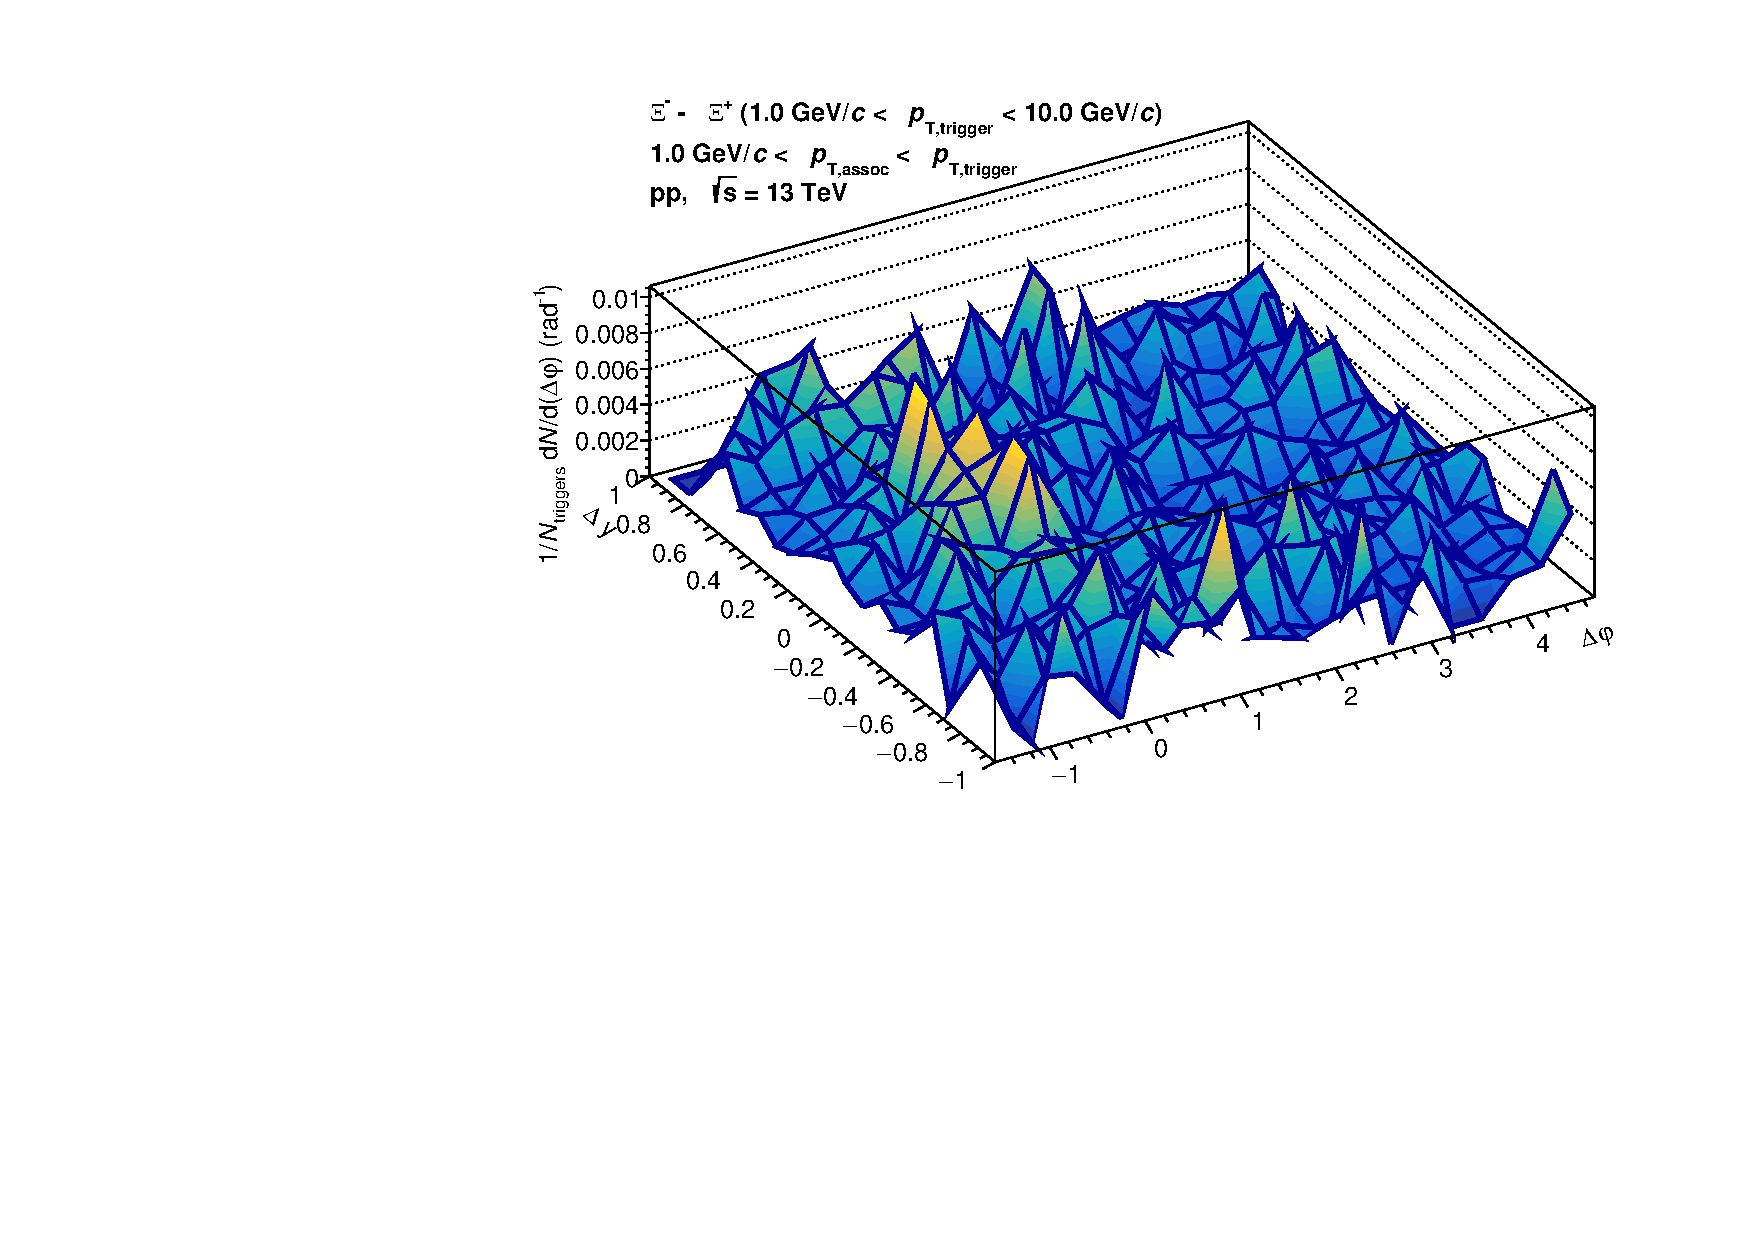
\includegraphics[width=\textwidth]{figures/Methodology/results/hXi-Xi+pT_1.0_10.0.pdf}
%     \caption{$\Xi^-$ - $\Xi^+$}
%     \label{fig:XiMinXiPlus}
%   \end{subfigure}
%   \hfill
%   \begin{subfigure}[t]{.49\textwidth}
%     \centering
%     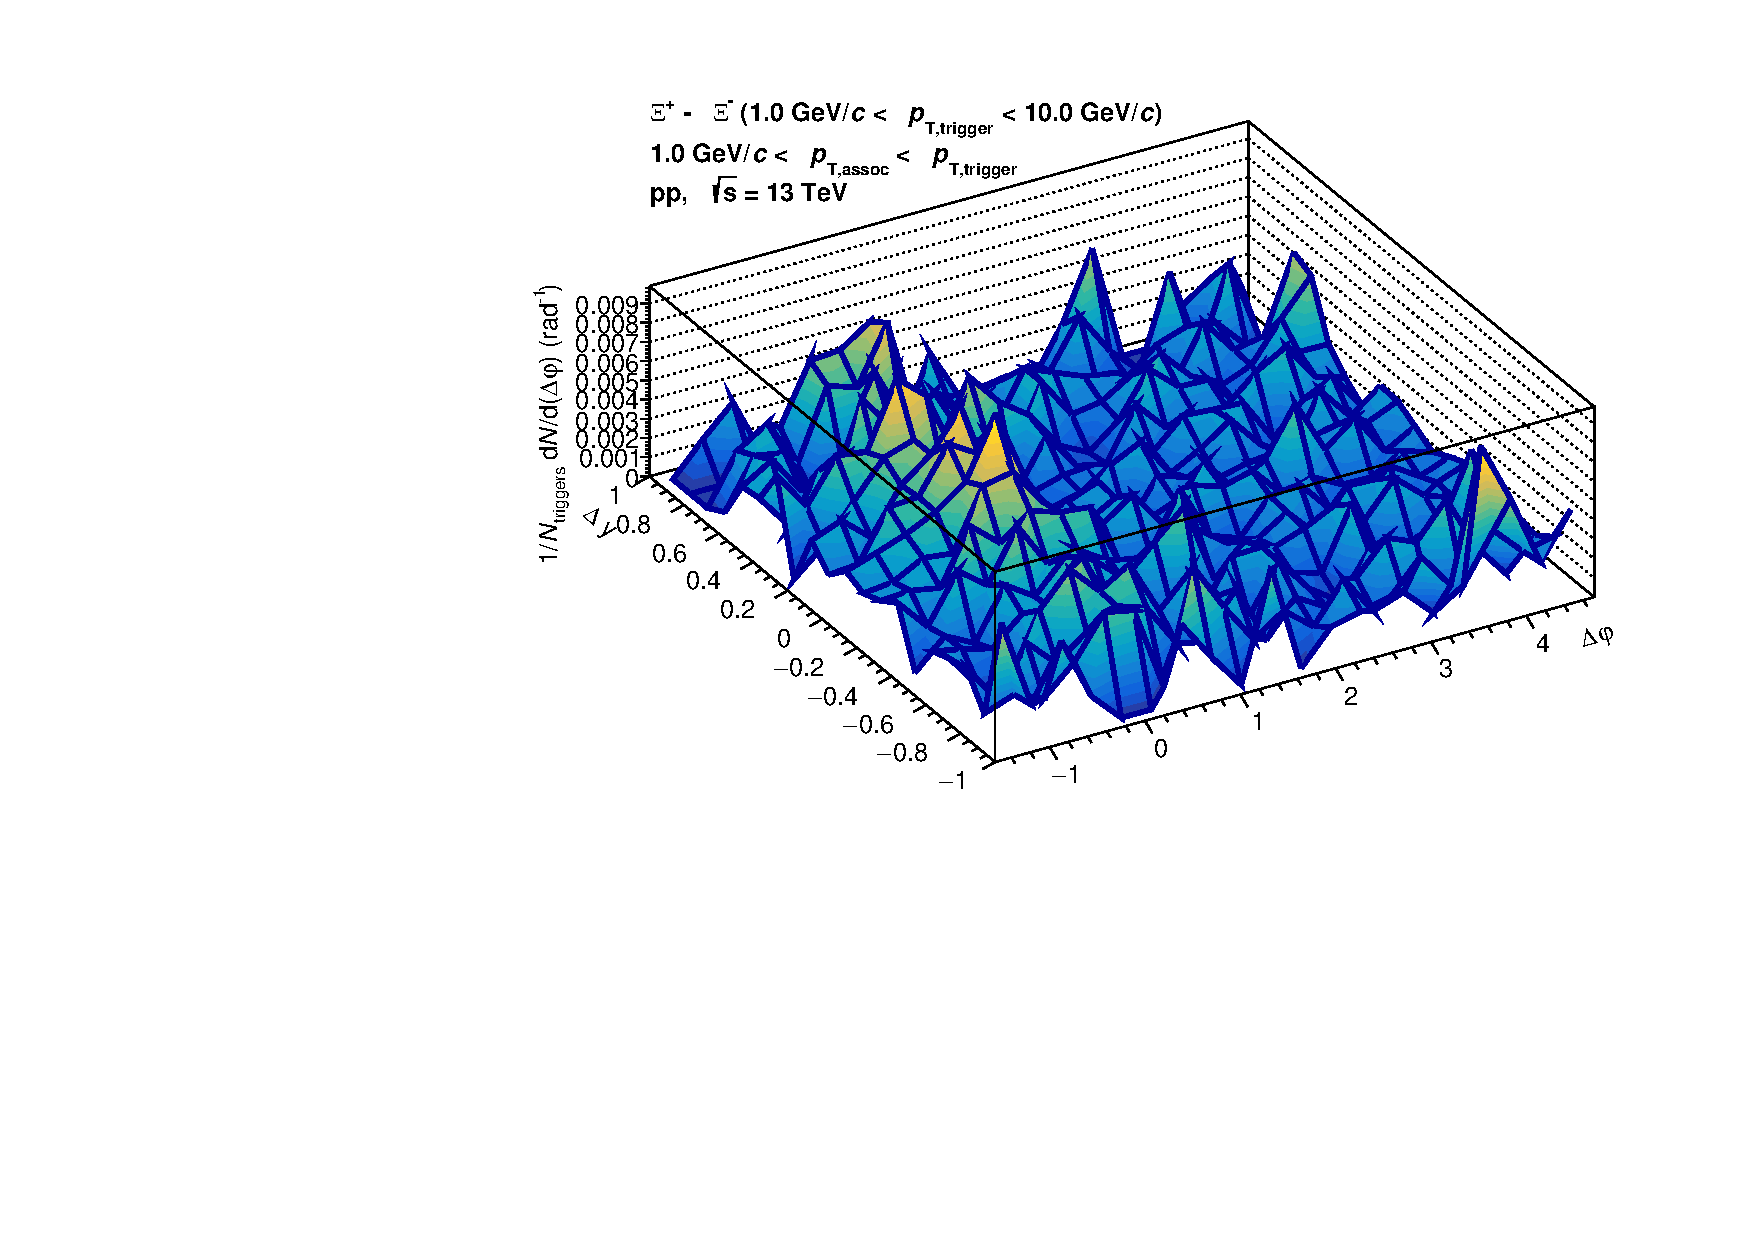
\includegraphics[width=\textwidth]{figures/Methodology/results/hXi+Xi-pT_1.0_10.0.pdf}
%     \caption{$\Xi^+$ - $\Xi^-$}
%     \label{fig:XiPlusXiMin}
%   \end{subfigure}
%   \begin{subfigure}[t]{.49\textwidth}
%     \centering
%     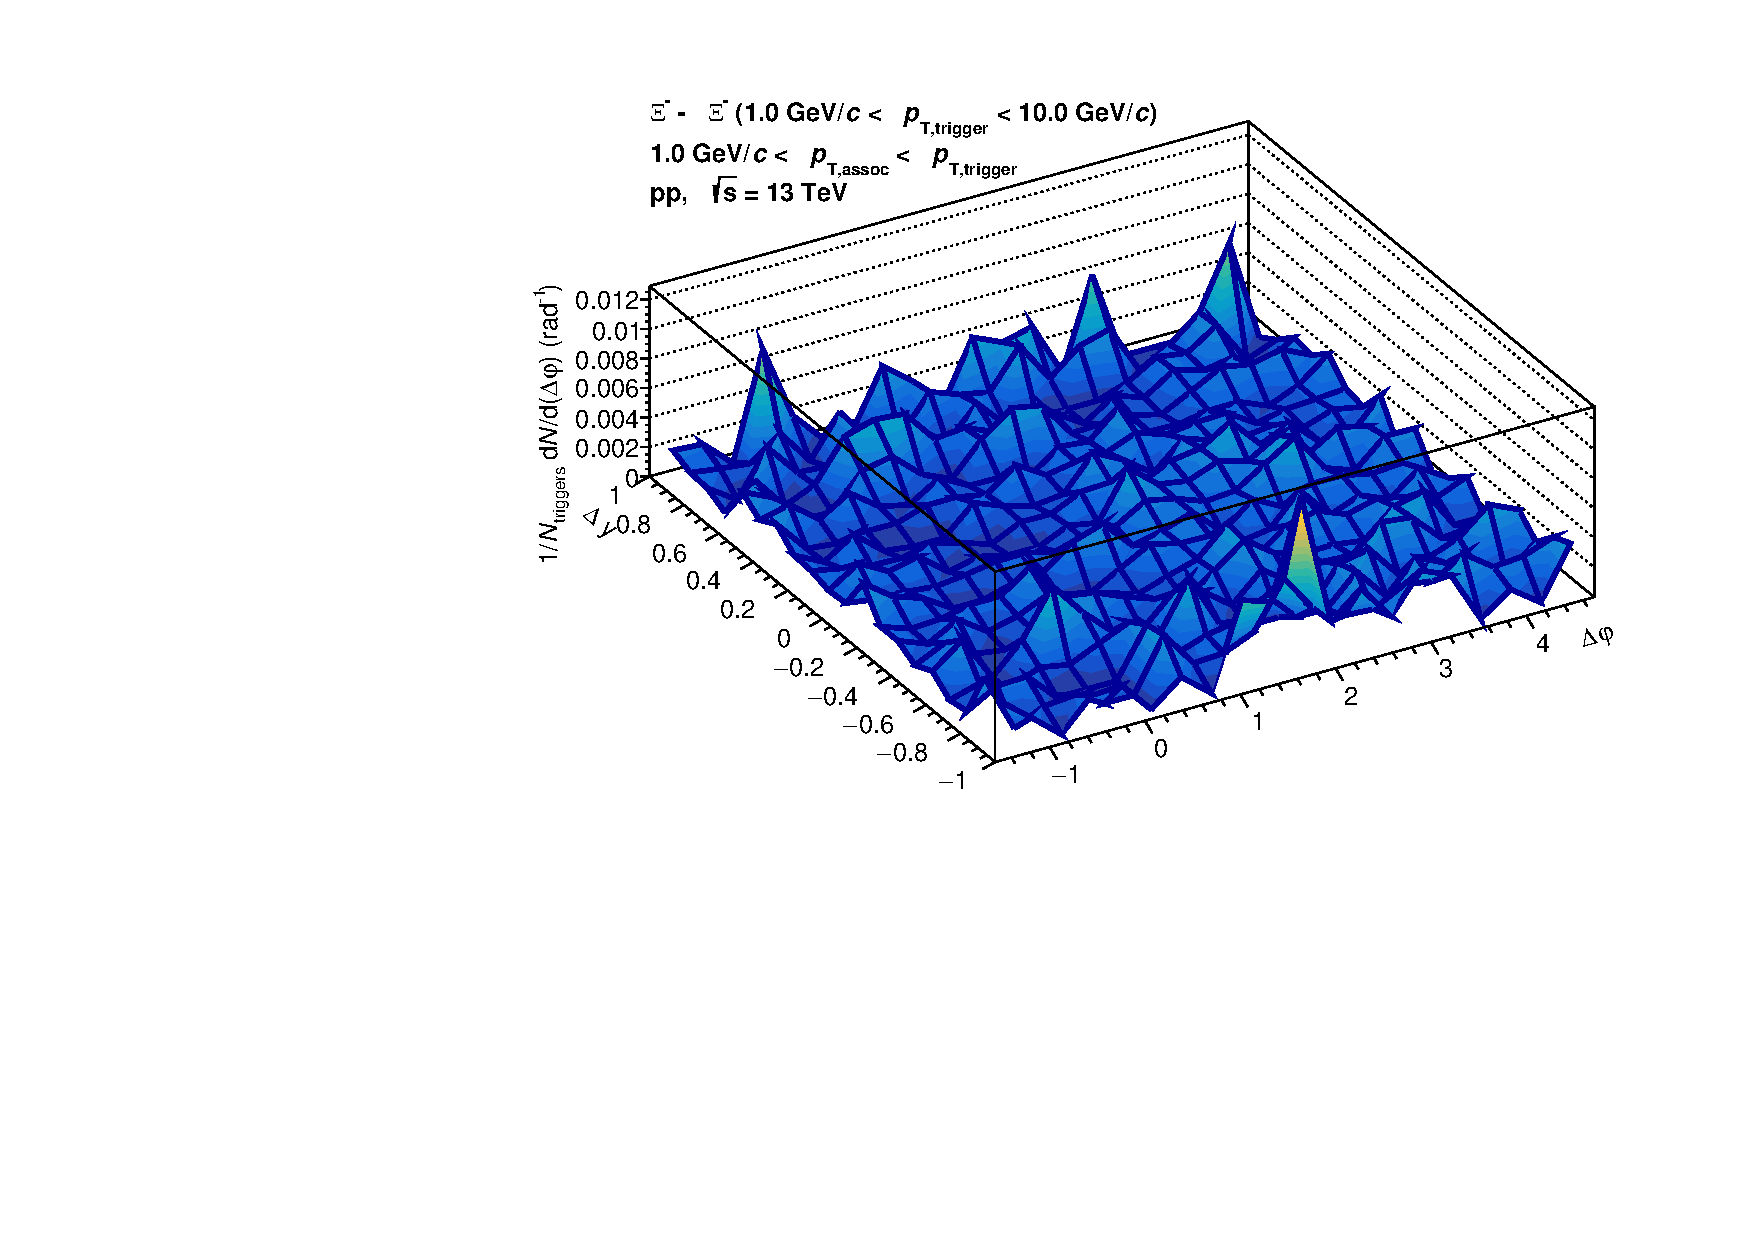
\includegraphics[width=\textwidth]{figures/Methodology/results/hXi-Xi-pT_1.0_10.0.pdf}
%     \caption{$\Xi^-$ - $\Xi^-$}
%     \label{fig:XiMinXiMin}
%   \end{subfigure}
%   \hfill
%   \begin{subfigure}[t]{.49\textwidth}
%     \centering
%     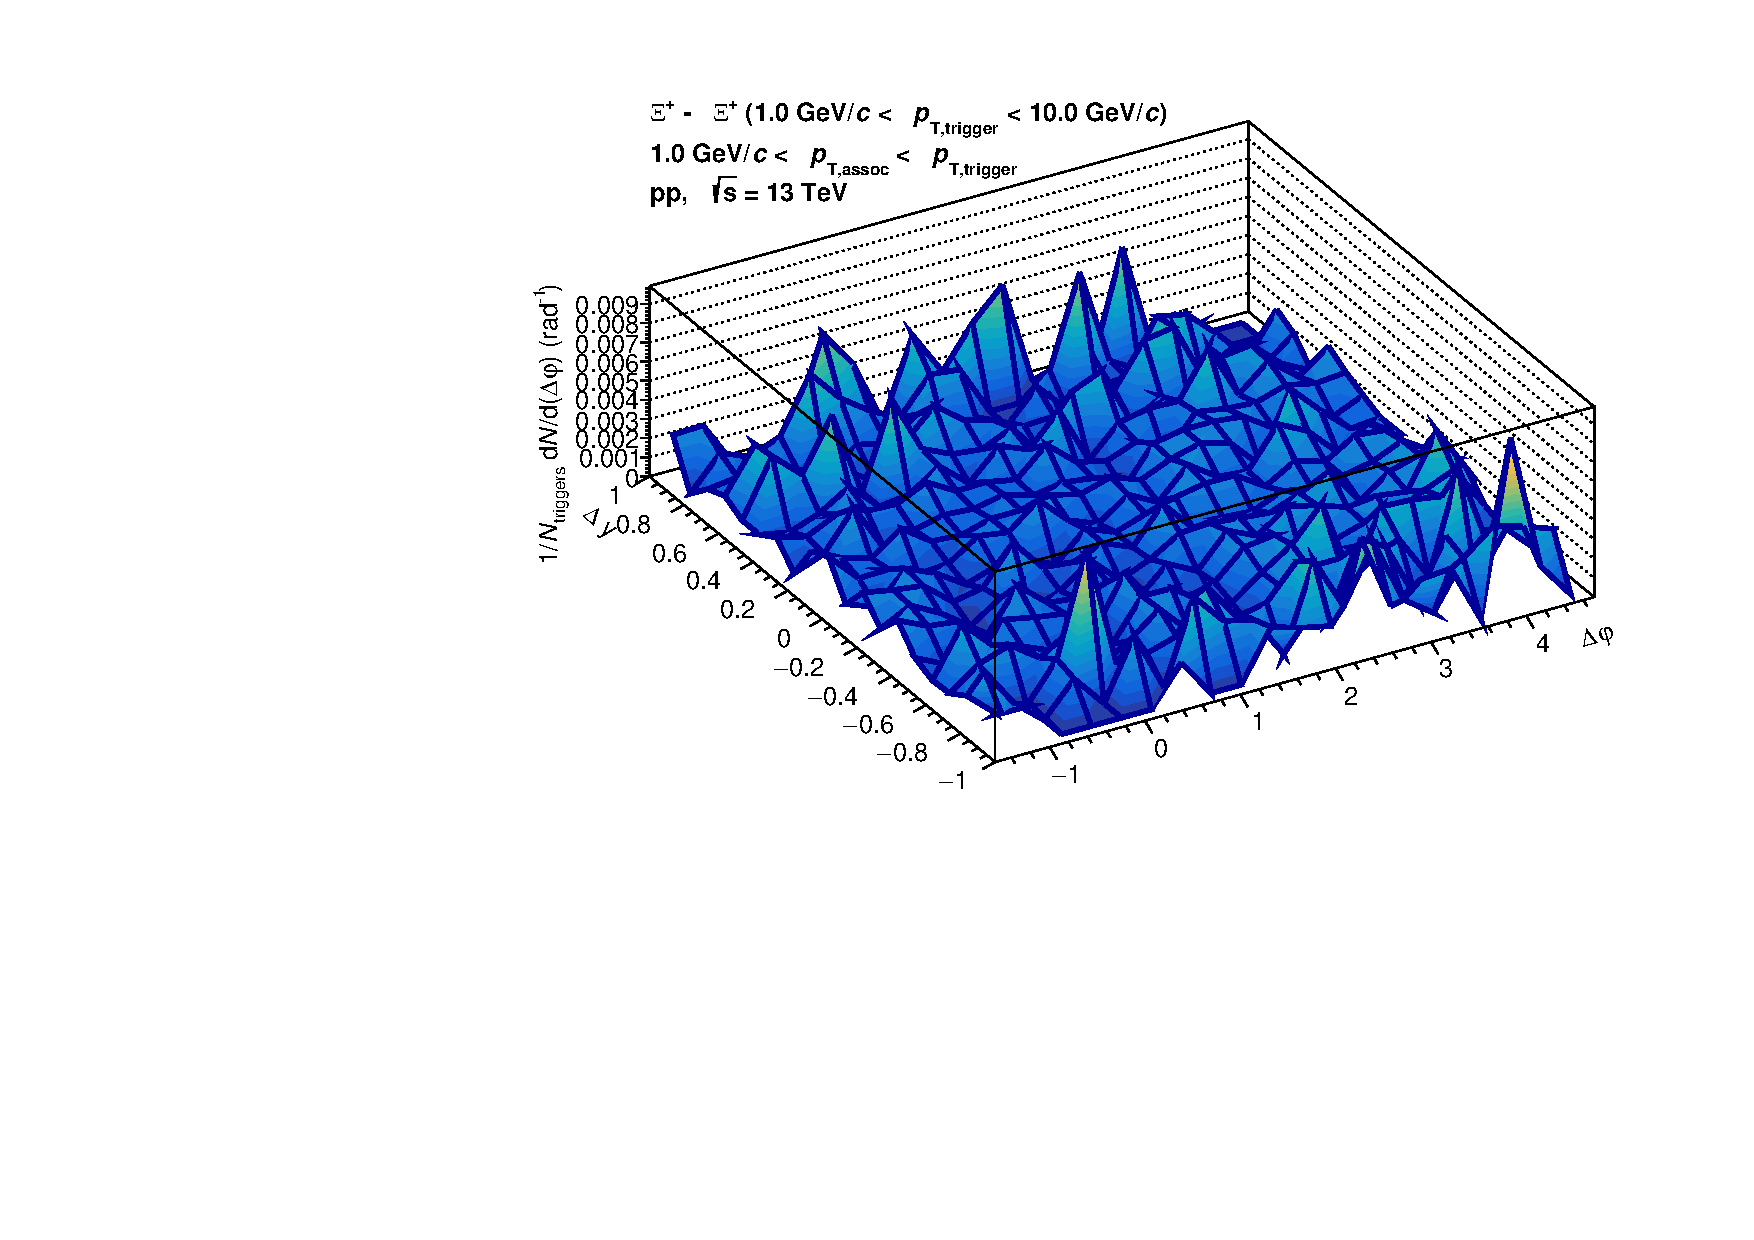
\includegraphics[width=\textwidth]{figures/Methodology/results/hXi+Xi+pT_1.0_10.0.pdf}
%     \caption{$\Xi^+$ - $\Xi^+$}
%     \label{fig:XiPlusXiPlus}
%   \end{subfigure}
%   \caption{\Xi\ - \Xi\ correlation results, split by sign combination}
%   \label{fig:resultssplit}
% \end{figure}

\begin{figure}[ht]
  \centering
  \begin{subfigure}[t]{.49\textwidth}
    \centering
    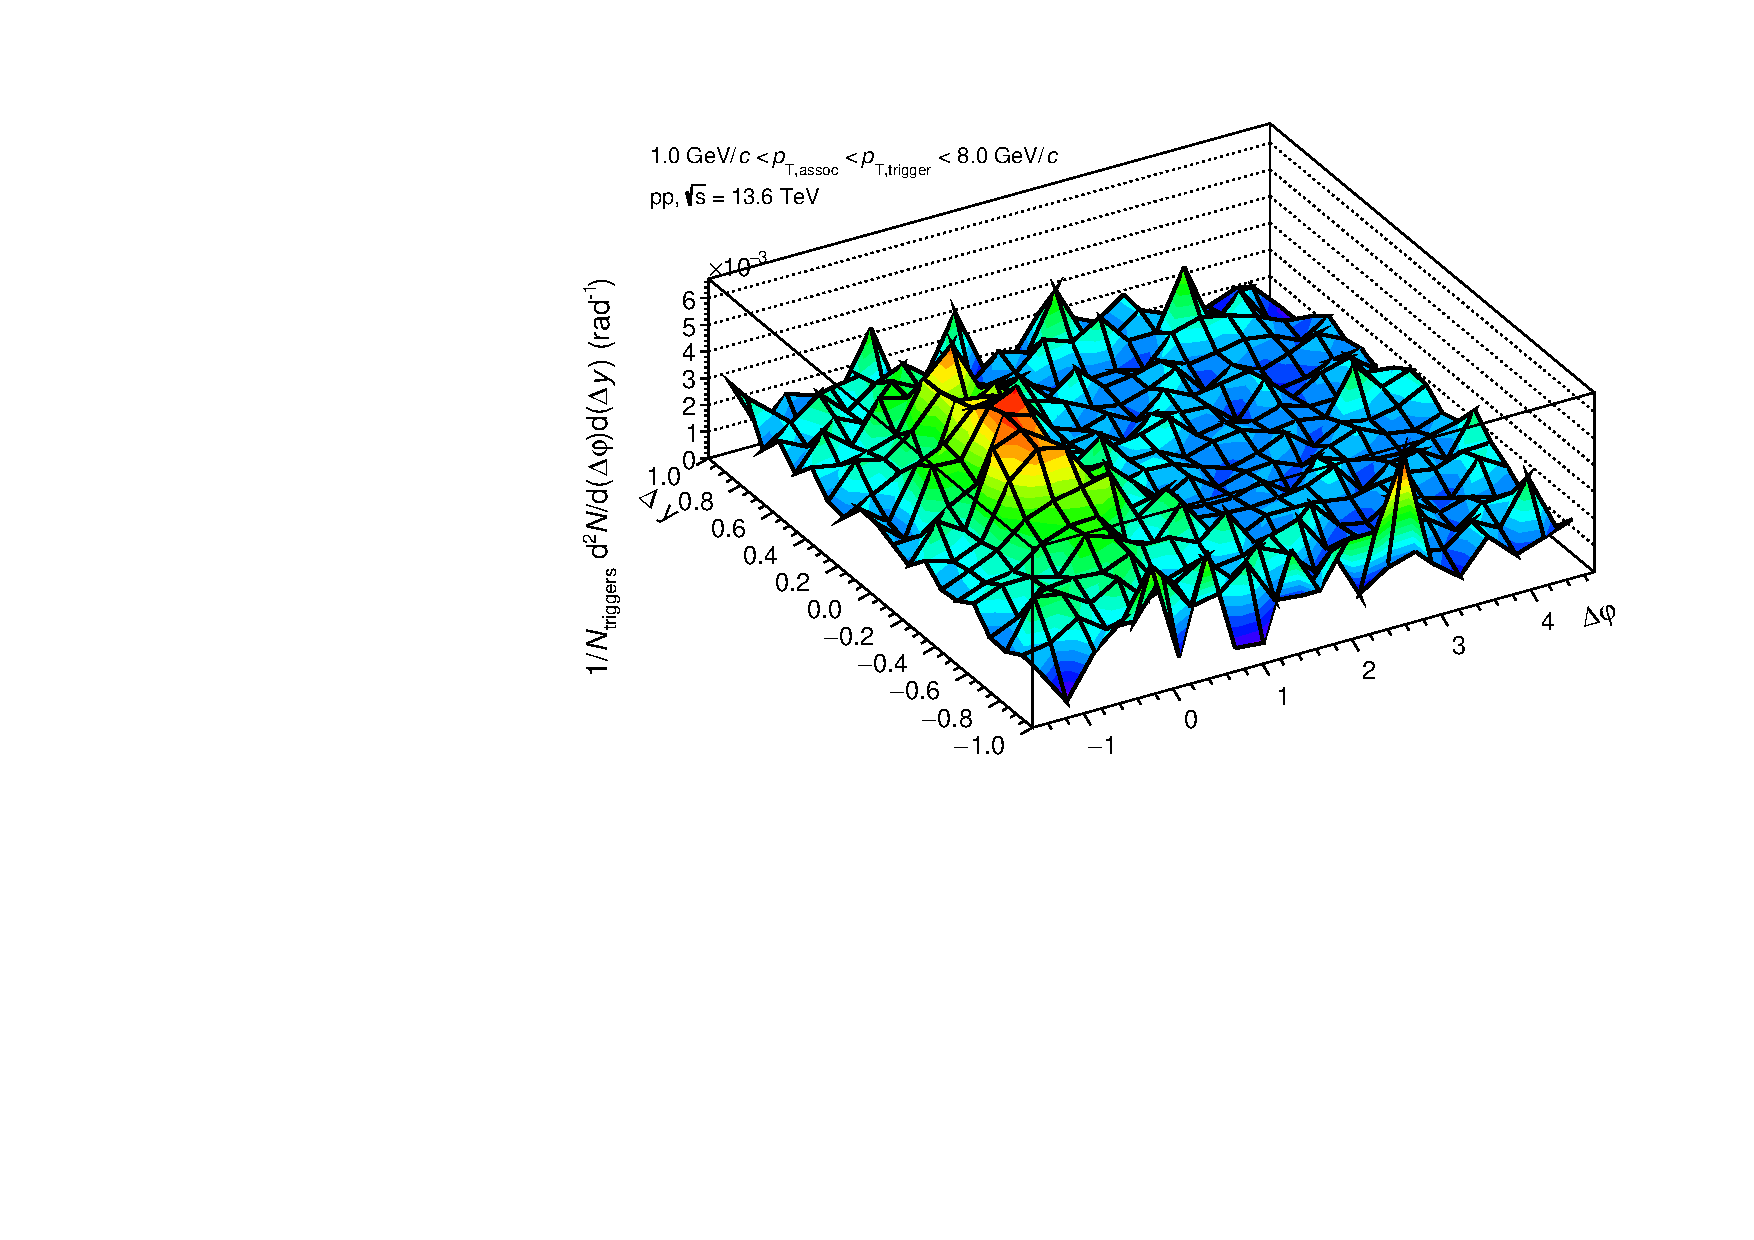
\includegraphics[width=\textwidth]{figures/Results/XiXi2DOS_pT_1.0_8.0.pdf}
    \caption{OS}
    \label{fig:XiXiOS}
  \end{subfigure}
  \hfill
  \begin{subfigure}[t]{.49\textwidth}
    \centering
    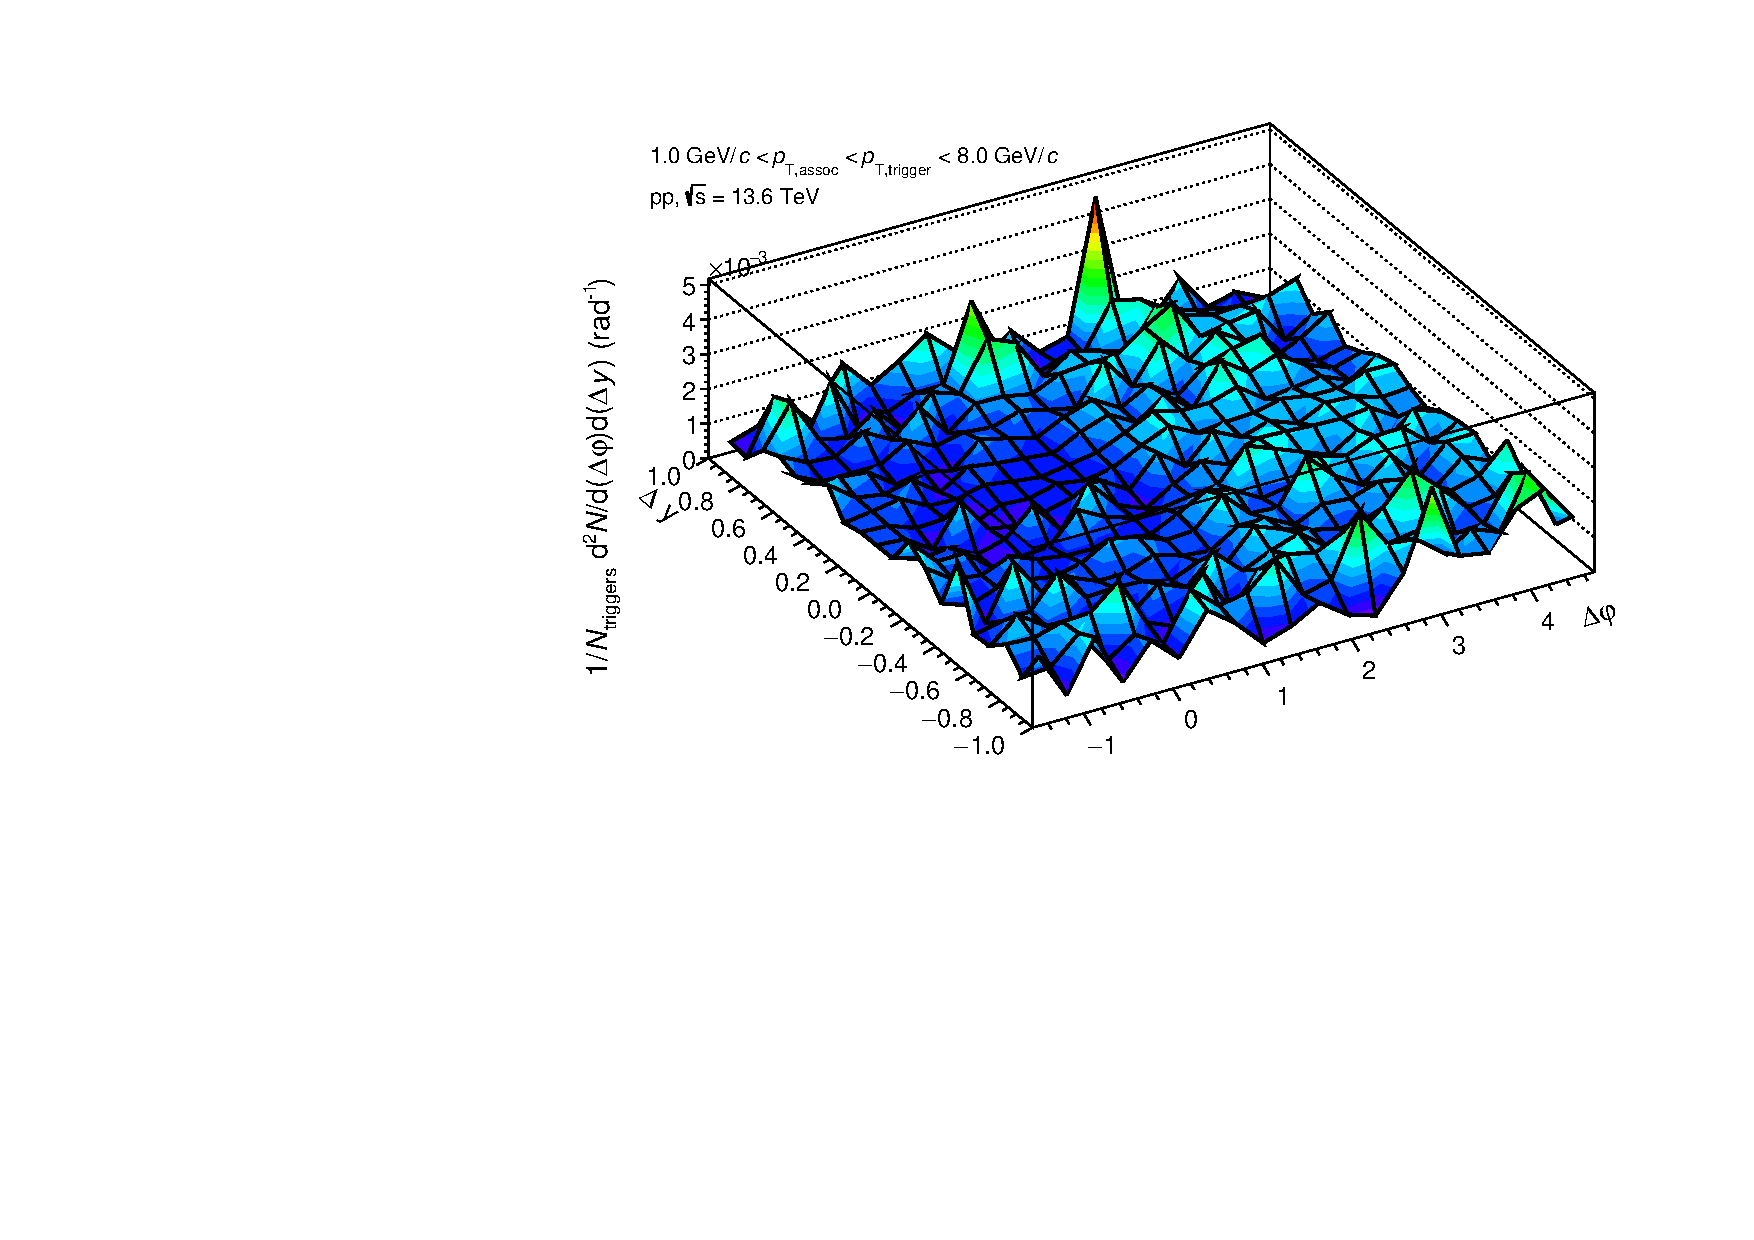
\includegraphics[width=\textwidth]{figures/Results/XiXi2DSS_pT_1.0_8.0.pdf}
    \caption{SS}
    \label{fig:XiXiSS}
  \end{subfigure}
  \begin{subfigure}[t]{.49\textwidth}
    \centering
    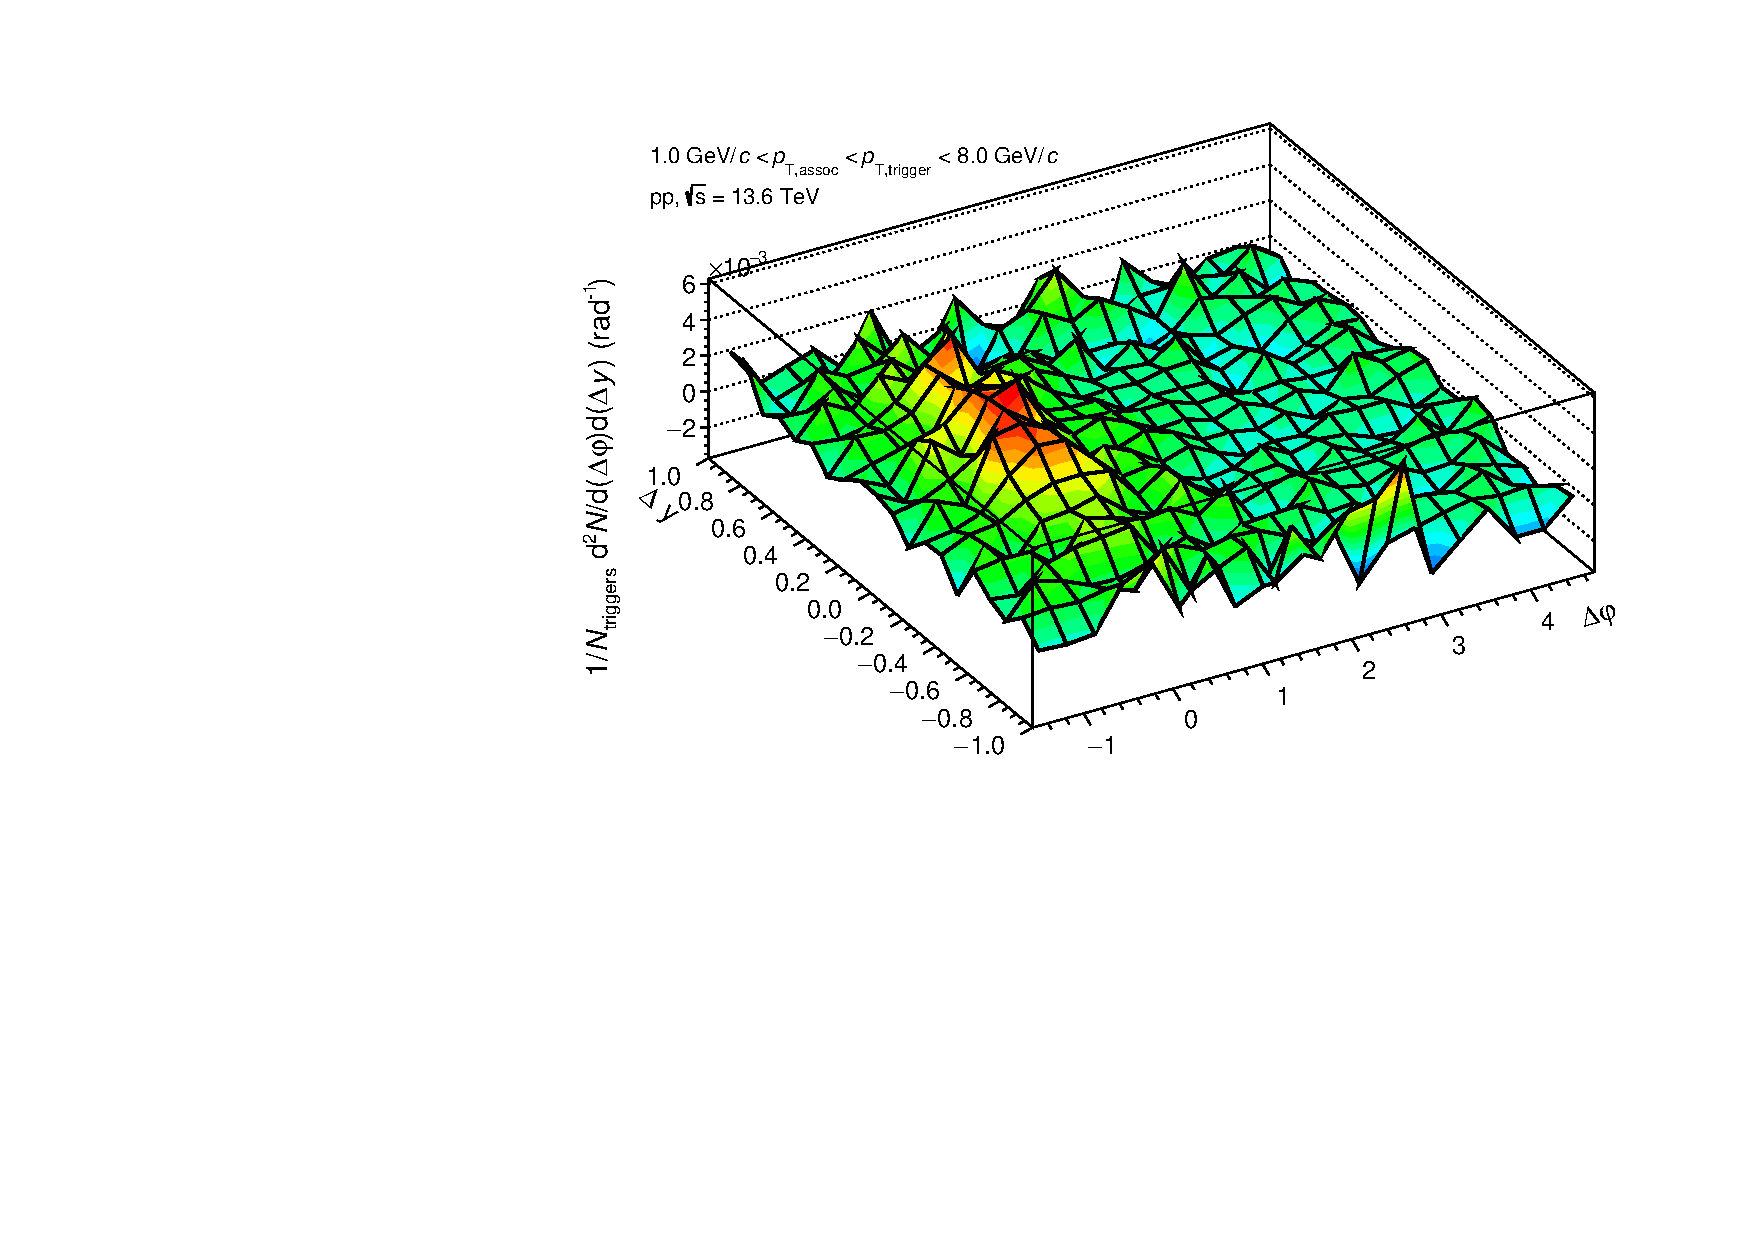
\includegraphics[width=\textwidth]{figures/Results/XiXi2DSub_pT_1.0_8.0.pdf}
    \caption{Subtracted}
    \label{fig:XiXiSub}
  \end{subfigure}
  \caption{\Xi\ - \Xi\ correlation results, combined into OS, SS, and subtracted \rs{I will probably put the 4 different sign combinations in the appendix, and just show the combined OS and SS here.}}
  \label{fig:resultscomb}
\end{figure}

The OS correlation (Figure \ref{fig:XiXiOS}) shows a clear near-side peak at $\Delta\varphi = 0$ and $\Delta y = 0$, on top of a flat pedestal. The near-side peak is a manifestation of quantum number conservation, namely strangeness and baryon number. The pedestal can be ascribed to uncorrelated production of \Xi\ baryons, and is described by the SS correlation function. Opposed to a near-side peak, the SS correlation function exhibits a near-side dip which has als been found in previous analyses on baryon-baryon correlations \cite{ALICE:angcorr}, indicating that the production of two \Xi\ (anti)baryons in close proximity is suppressed. In both correlation functions one can see rather large fluctuations at the edges of the \dy\ range, which are due to the large ME corrections in these regions. The Balance function described by the OS correlation function subtracted by the SS correlation function also shows a clear near-side peak, propagated through from the OS correlation function, while the pedestal is largely subtracted away. \rs{mention (probably later) mechanisms for e.g. back-to-back production of \Xi\ pairs (initial hard scattering), and that they should be present in both OS and SS, thus subtracted away in the Balance Function.}

The 1D projections onto \dphi\ are shown in Figure \ref{fig:Results1D}, where the bars represent the statistical uncertainties and the shaded boxes represent the systematic uncertainties. \rs{these plots are copied from the spectra chapter, where we have outlined the systematic uncertainty procedure. We should reorganise it so that the systematic uncertainty procedure is outlined here.} For the OS correlation function the near-side peak is clearly visible, on top of the aforementioned pedestal. The SS correlation function again shows a near-side dip, but more interestingly on the away-side the pedestal seems to be at a slightly lower level than for the OS correlation function. This is verified by the subtracted balance function, where all datapoints lie above the x-axis. This shows that, while the vast majority of the strangeness is balanced locally, some of it is balanced at larger \dphi\ values. 

\begin{figure}[ht!]
  \centering
  \begin{subfigure}[t]{.49\textwidth}
    \centering
    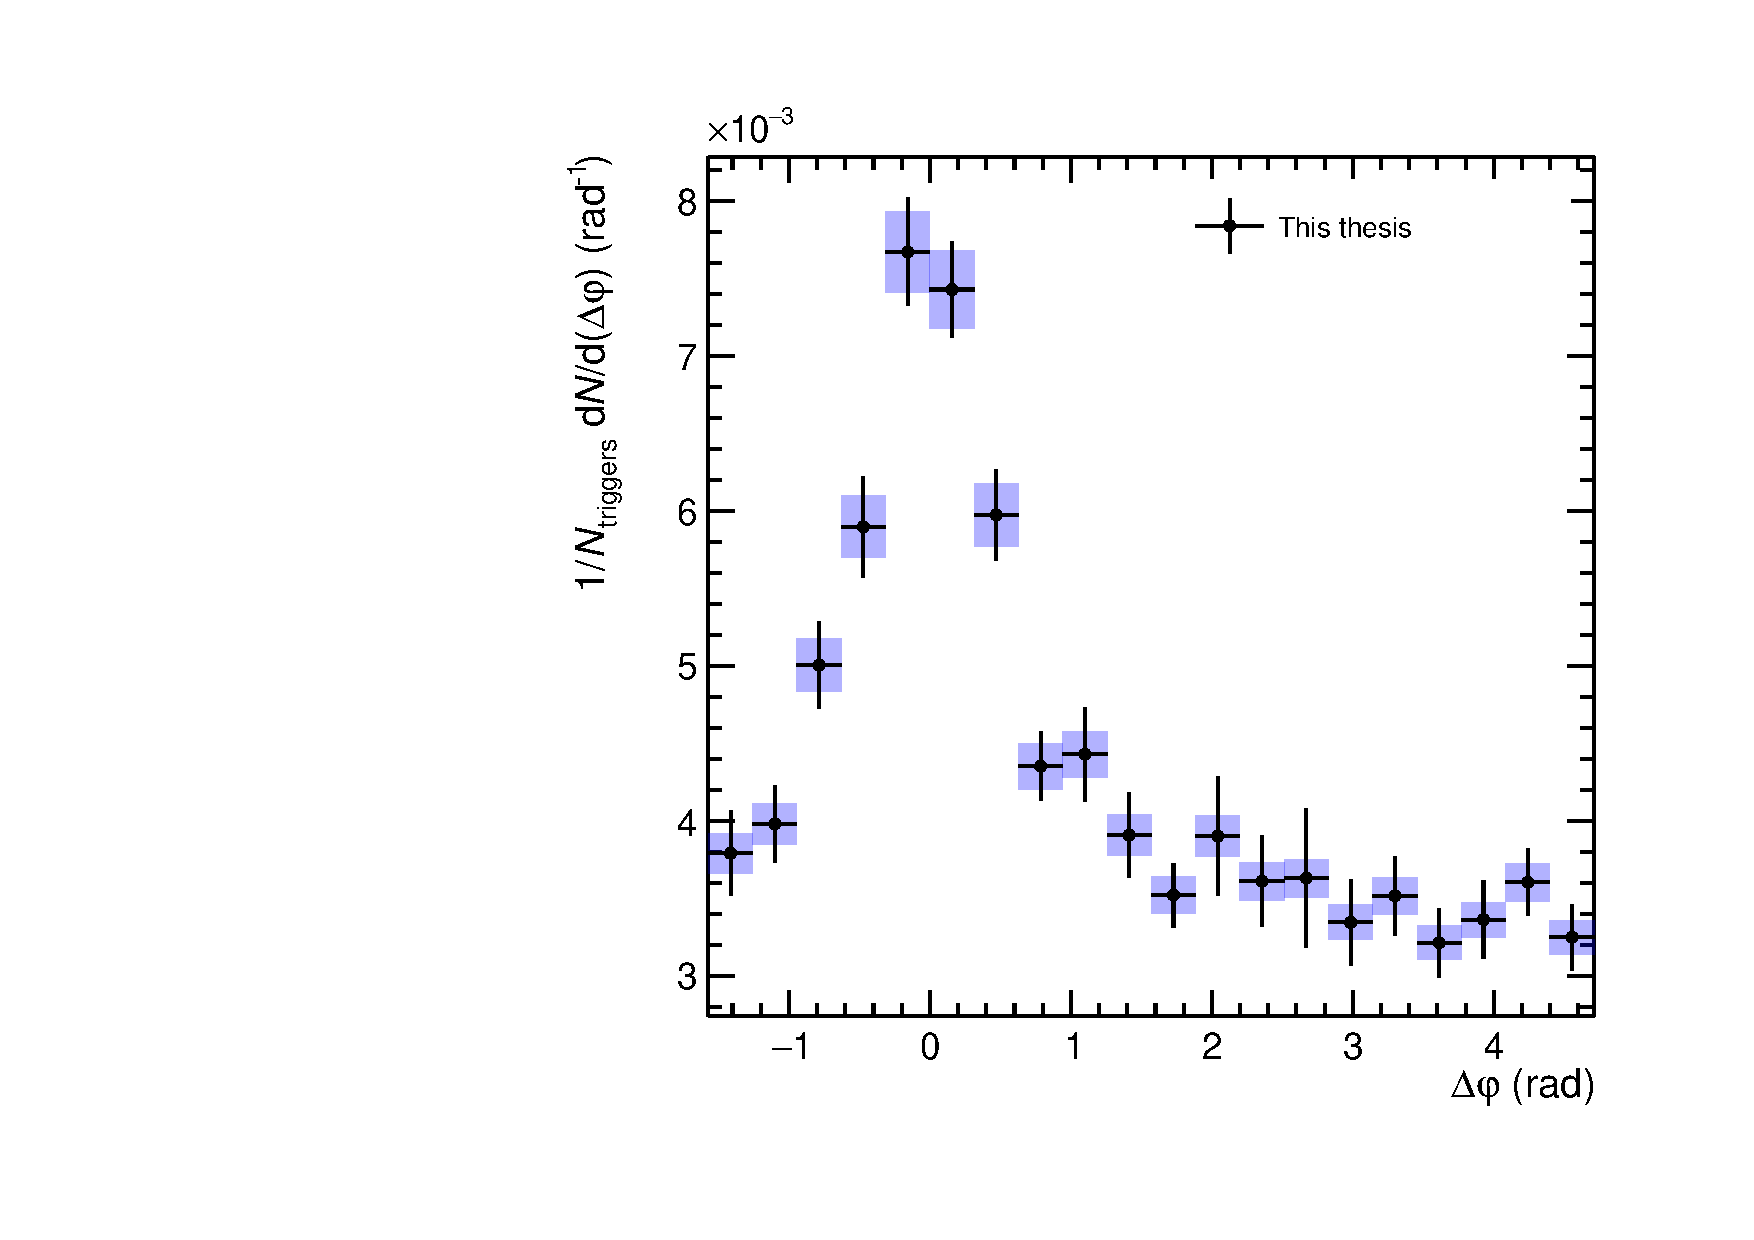
\includegraphics[width=\textwidth]{figures/systematics/systematics_OS.pdf}
    \caption{Per trigger yield of OS \Xi\ - \Xi\ pairs as a function of \dphi. }
    \label{fig:ResultsOS1D}
  \end{subfigure}
  \hfill
  \begin{subfigure}[t]{.49\textwidth}
    \centering
    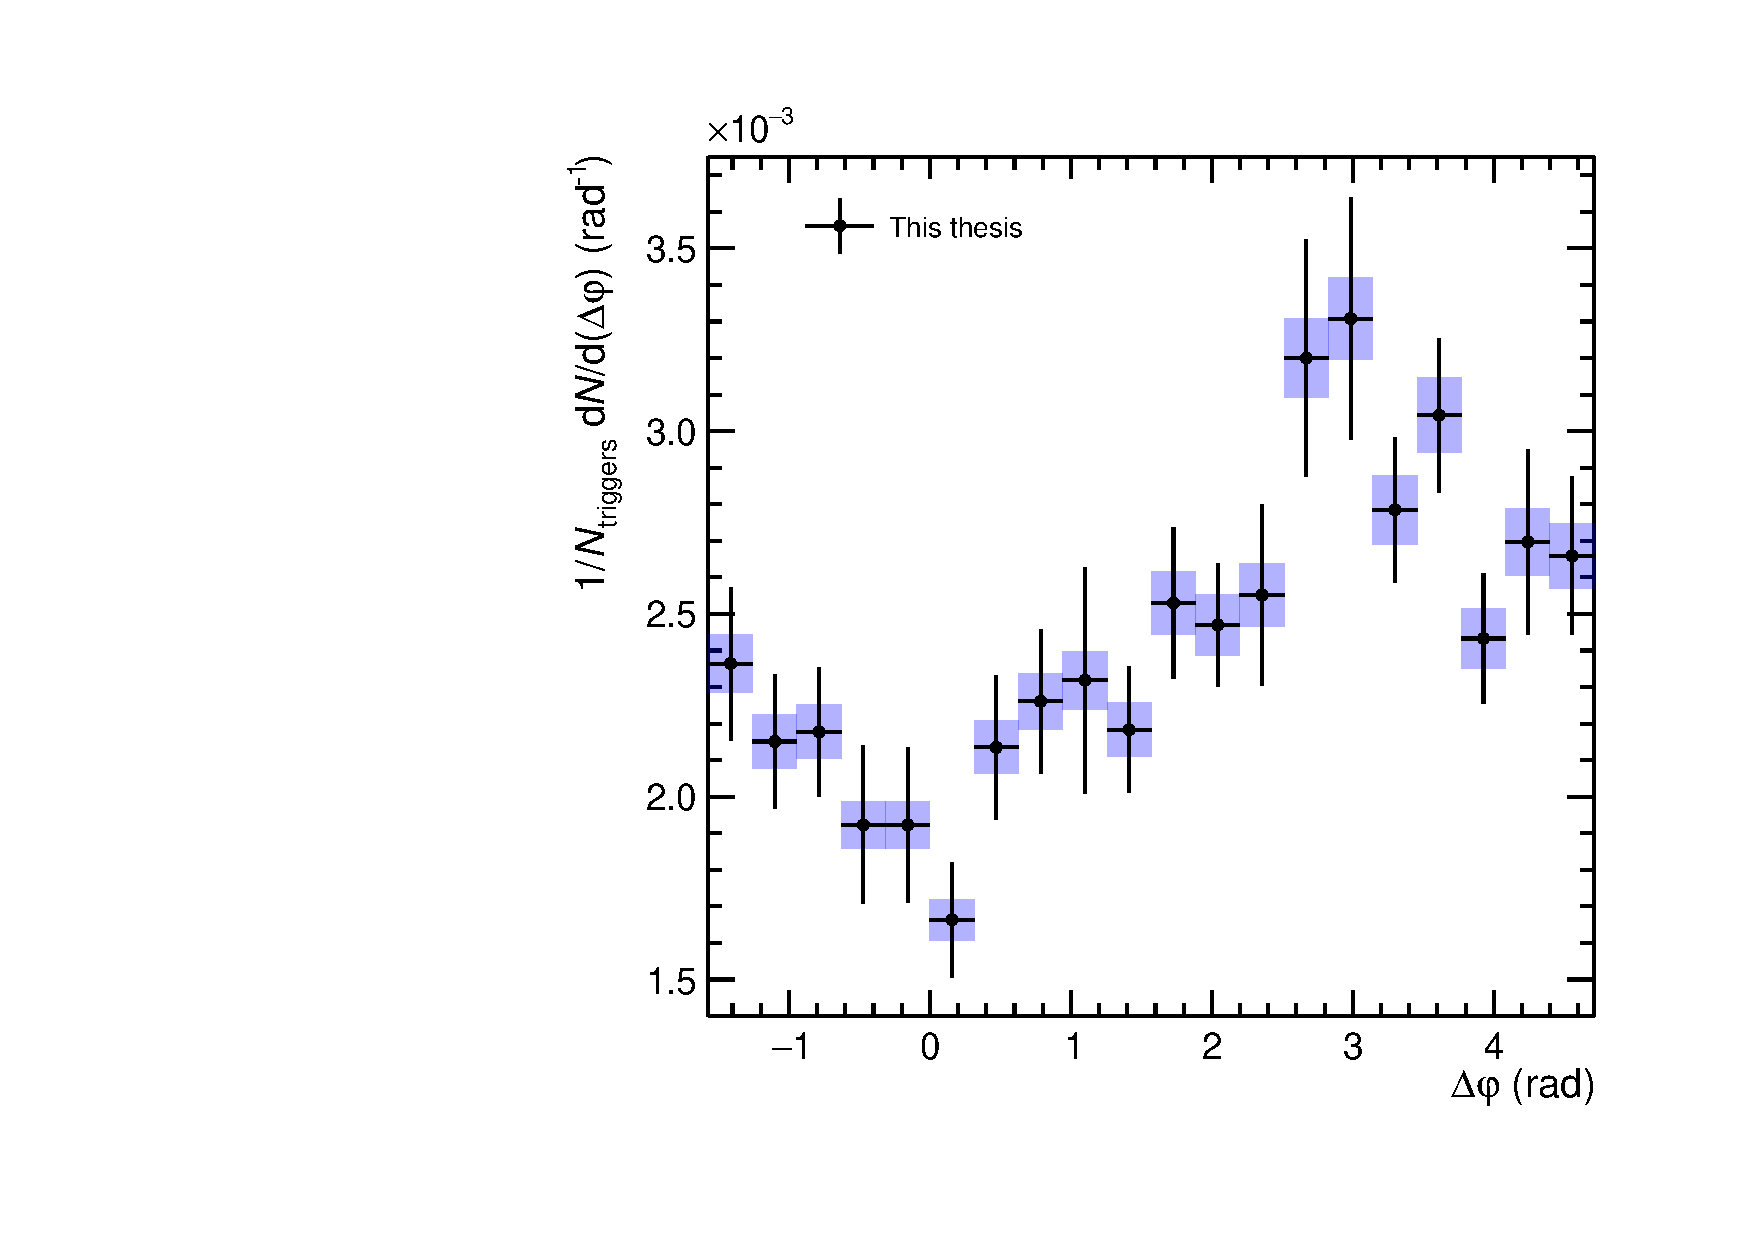
\includegraphics[width=\textwidth]{figures/systematics/systematics_SS.pdf}
    \caption{Per trigger yield of SS \Xi\ - \Xi\ pairs as a function of \dphi. }
    \label{fig:ResultsSS1D}
  \end{subfigure}
  \hfill
  \begin{subfigure}[t]{.49\textwidth}
    \centering
    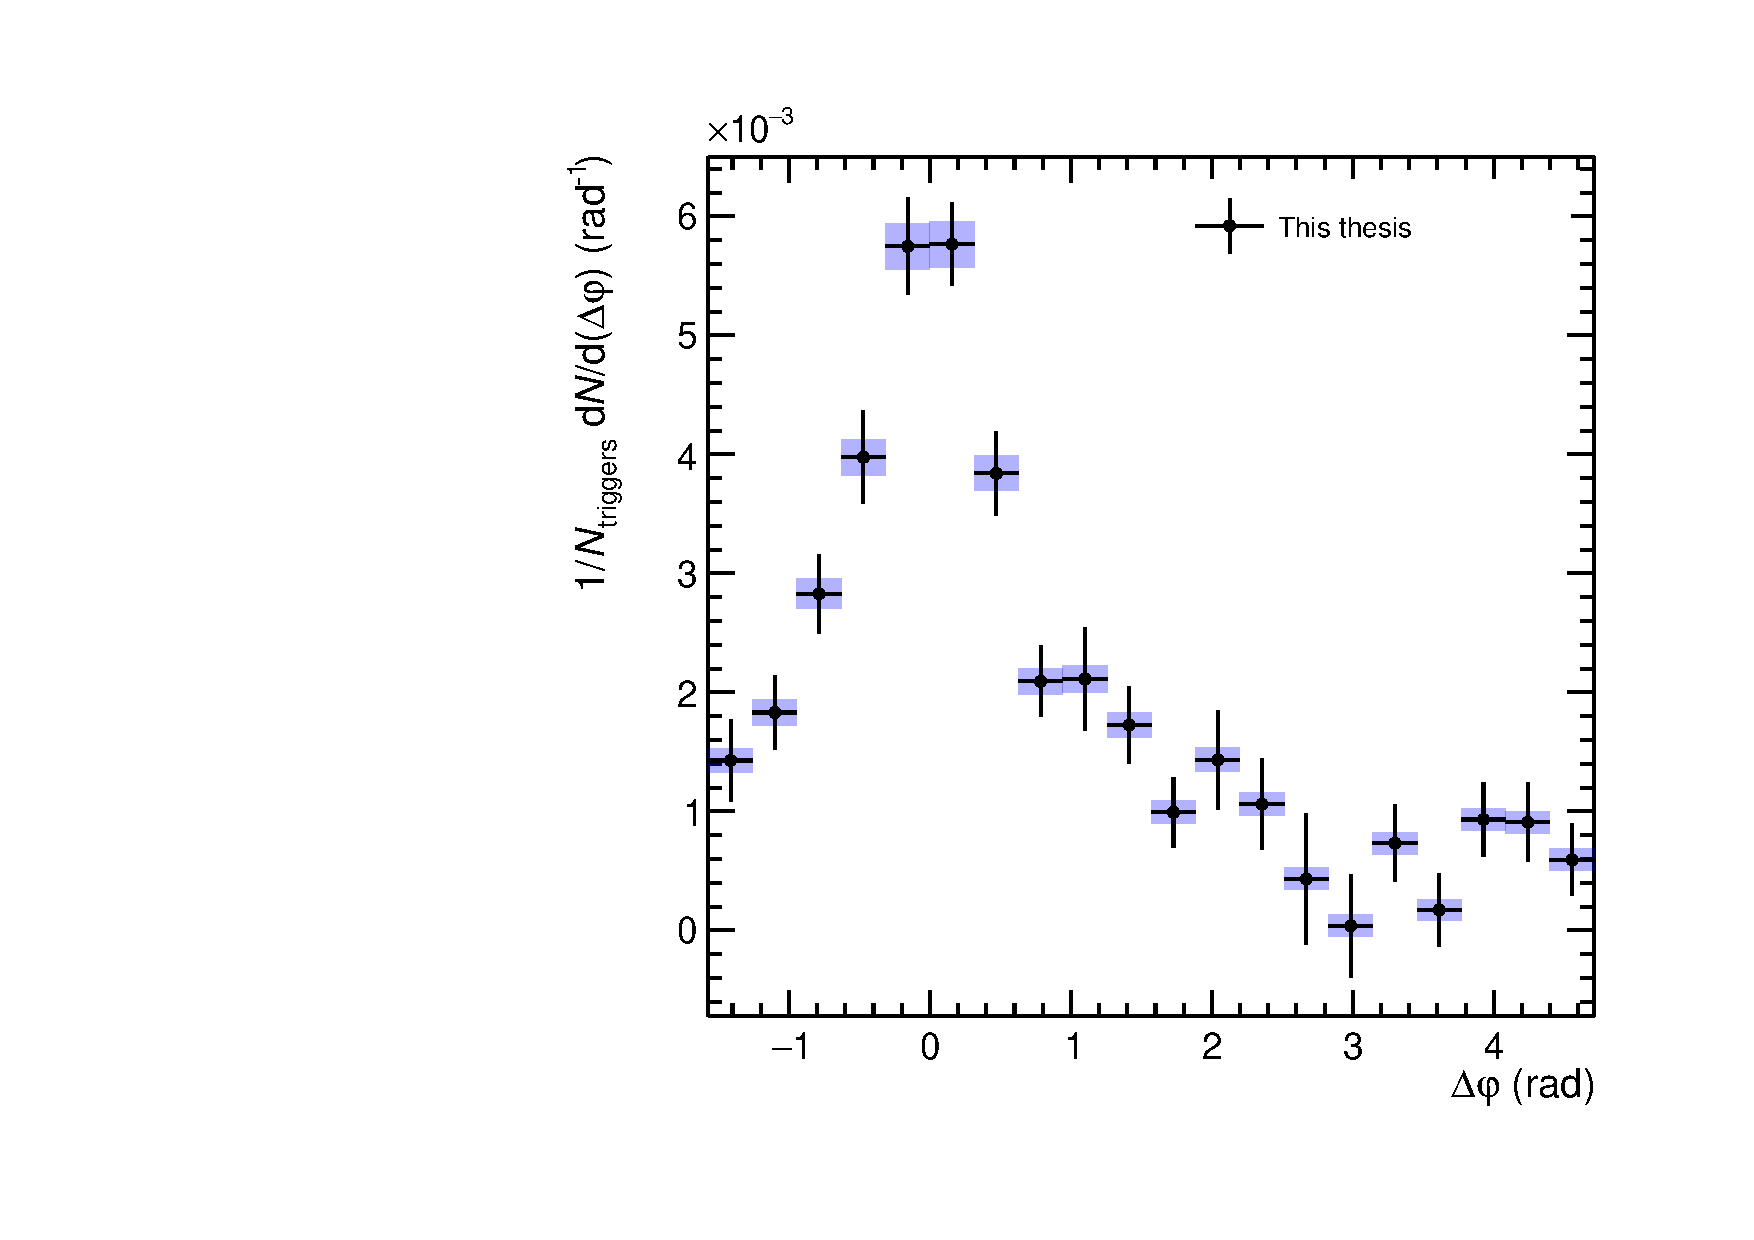
\includegraphics[width=\textwidth]{figures/systematics/systematics_Sub.pdf}
    \caption{Per trigger yield of OS - SS \Xi\ - \Xi\ pairs as a function of \dphi. }
    \label{fig:ResultsSub1D}
  \end{subfigure}
  \caption{Per trigger yield of OS, SS, and OS - SS \Xi\ - \Xi\ pairs as a function of \dphi, with statistical and systematic uncertainties. \rs{make the text in the plots so we can remove the subcaptions}}
  \label{fig:Results1D}
\end{figure}

% As we've already shown the comparisons at the start of the spectra chapter, probably remove them here. we can return to them in the discussion section. 
% \begin{figure}[ht]
%   \centering
%   \begin{subfigure}[t]{.49\textwidth}
%     \centering
%     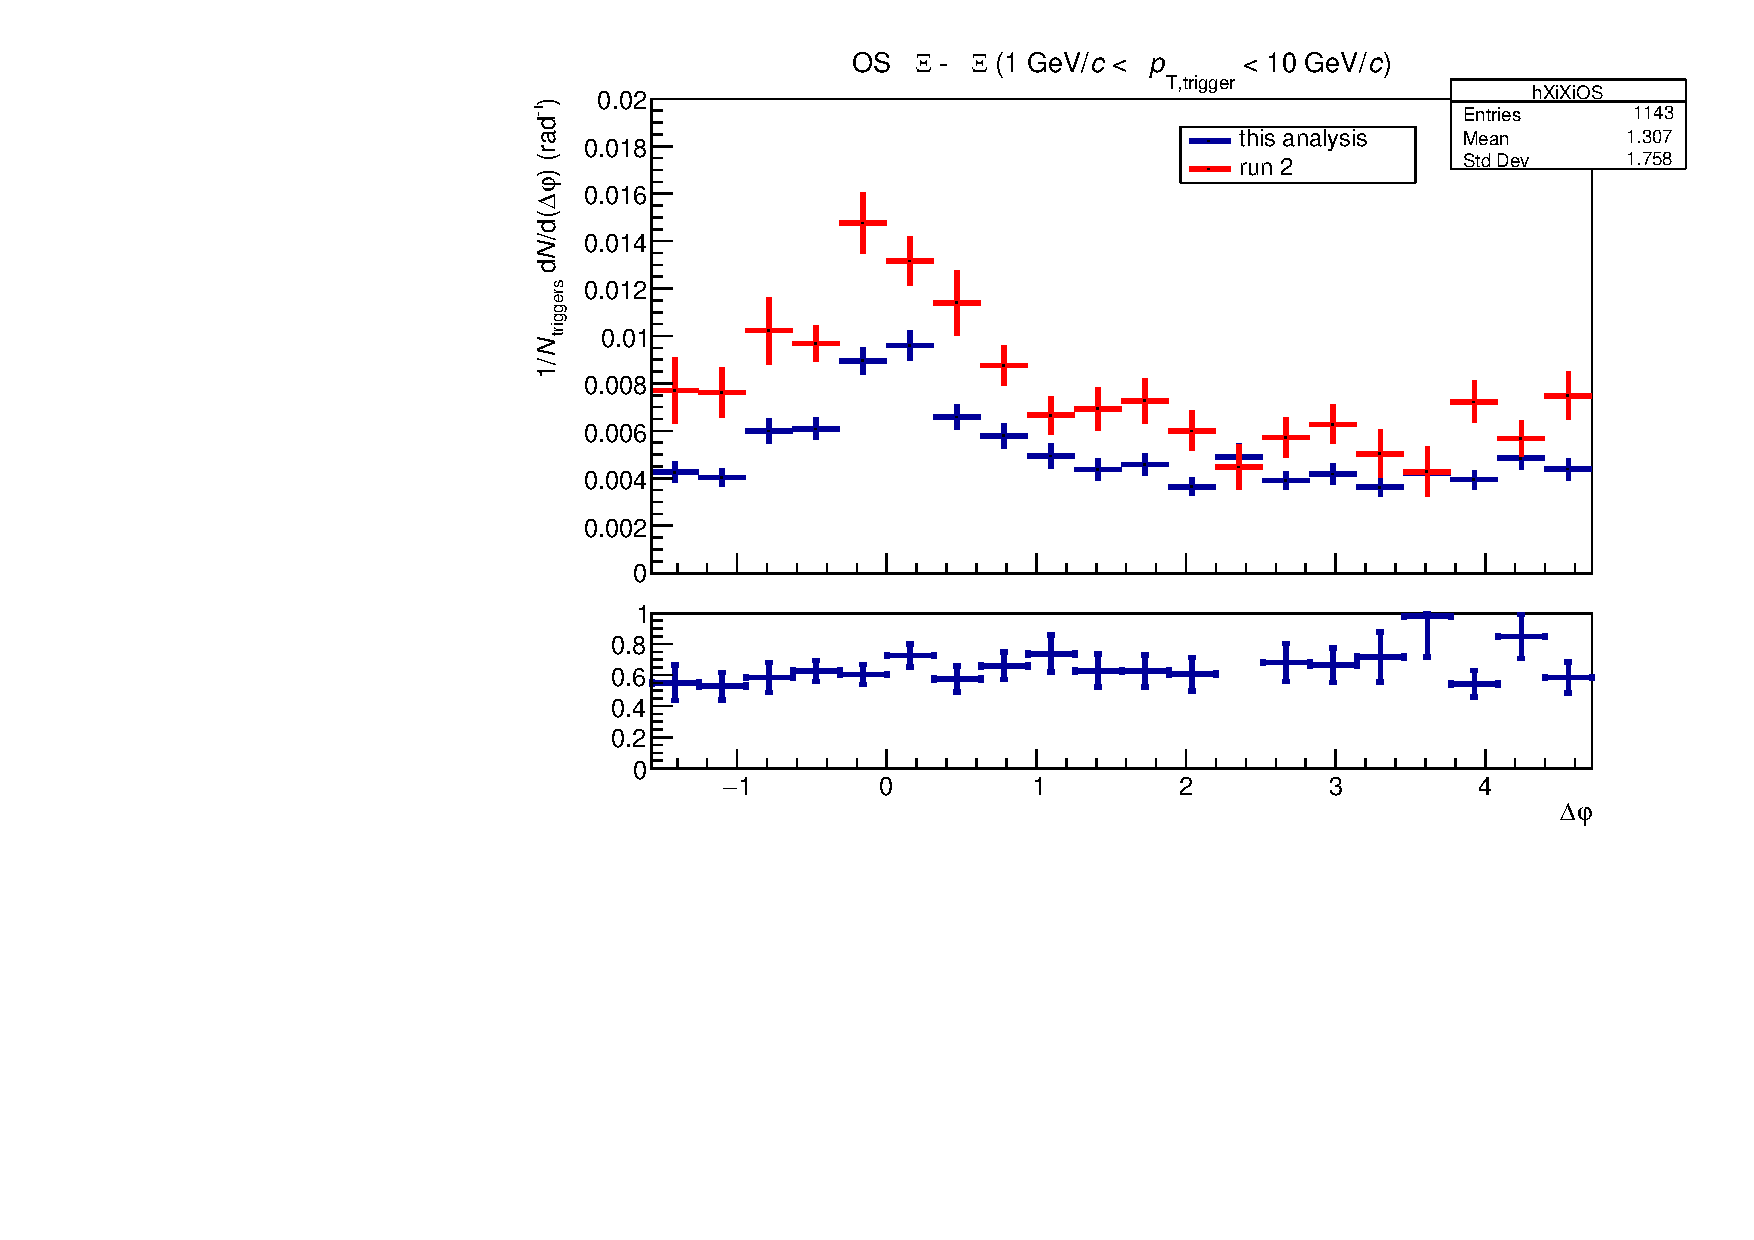
\includegraphics[width=\textwidth]{figures/Methodology/OSRatio.pdf}
%     \caption{OS}
%     \label{fig:XiXiOS1D}
%   \end{subfigure}
%   \hfill
%   \begin{subfigure}[t]{.49\textwidth}
%     \centering
%     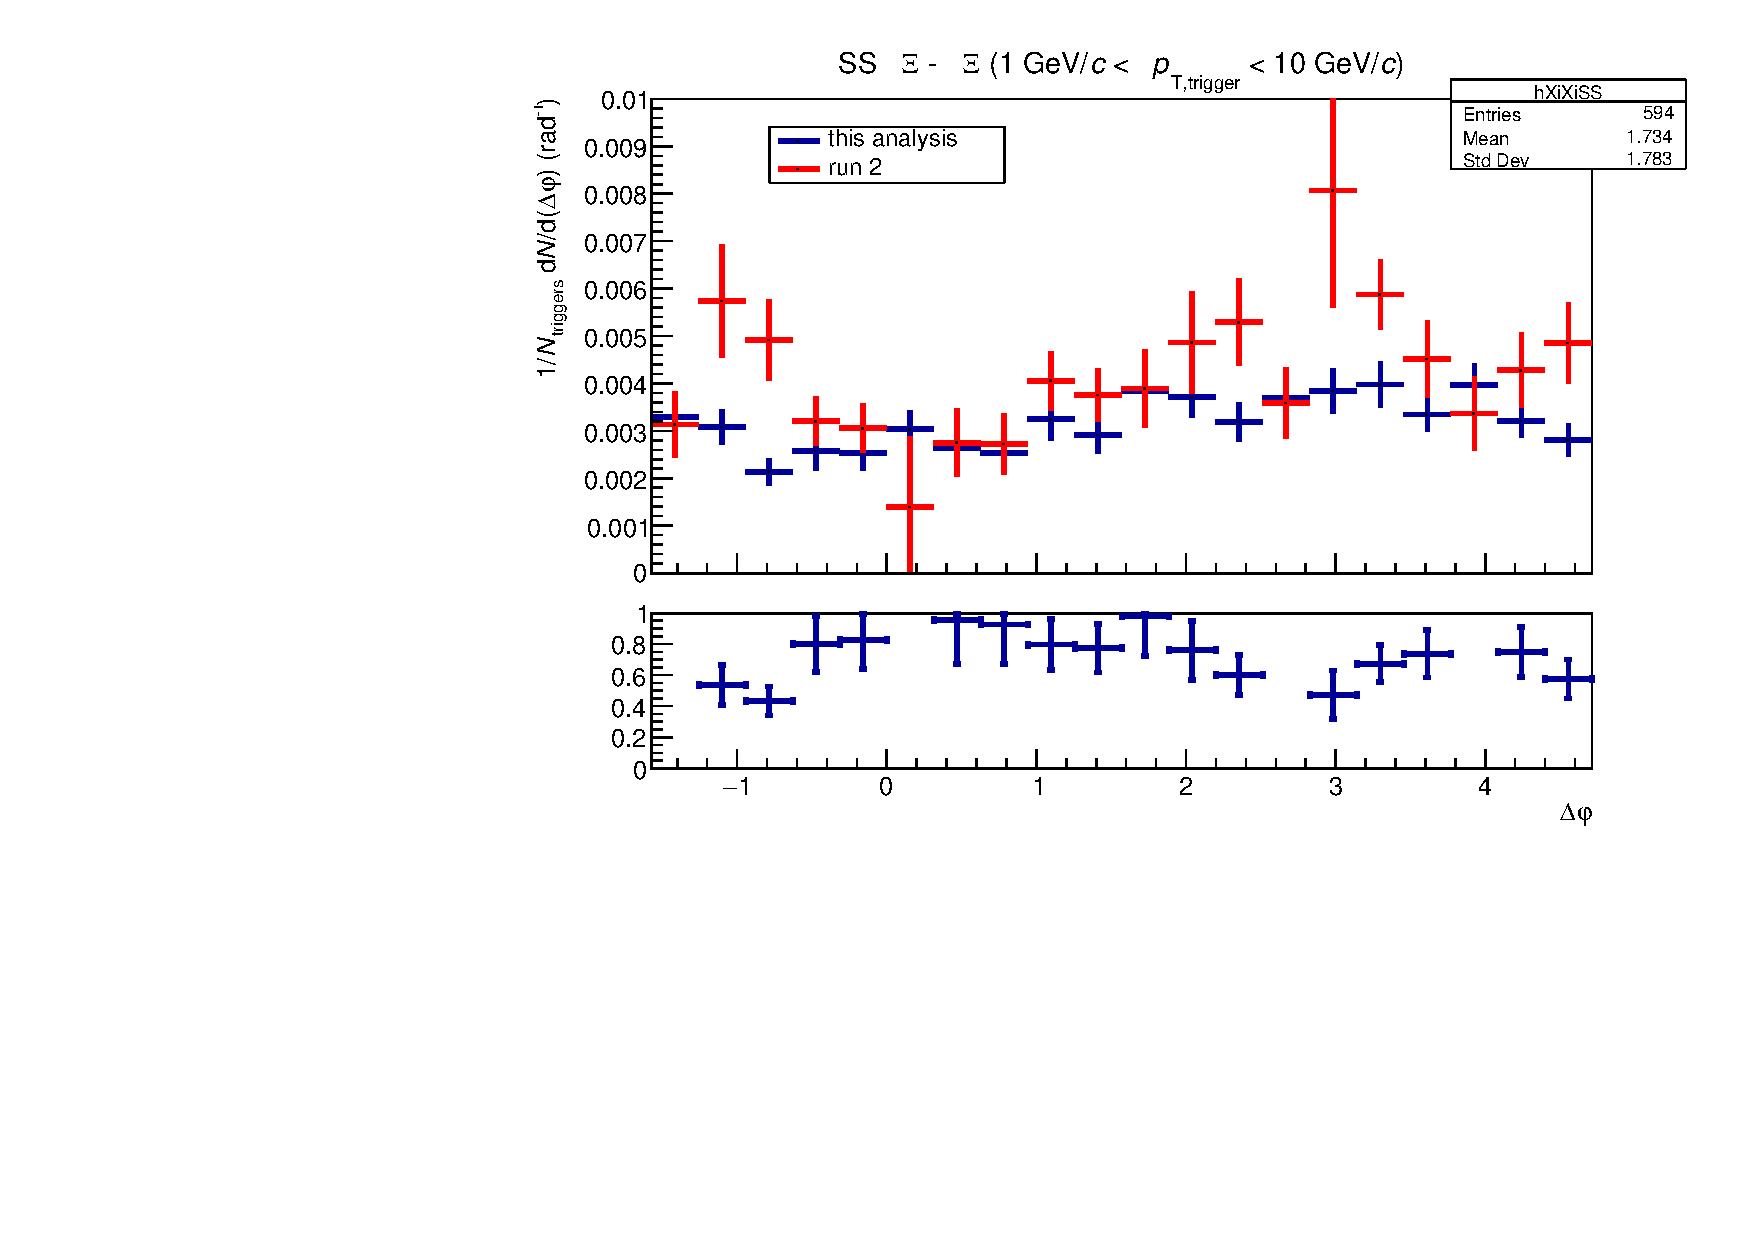
\includegraphics[width=\textwidth]{figures/Methodology/SSRatio.pdf}
%     \caption{SS}
%     \label{fig:XiXiSS1D}
%   \end{subfigure}
%   \begin{subfigure}[t]{.49\textwidth}
%     \centering
%     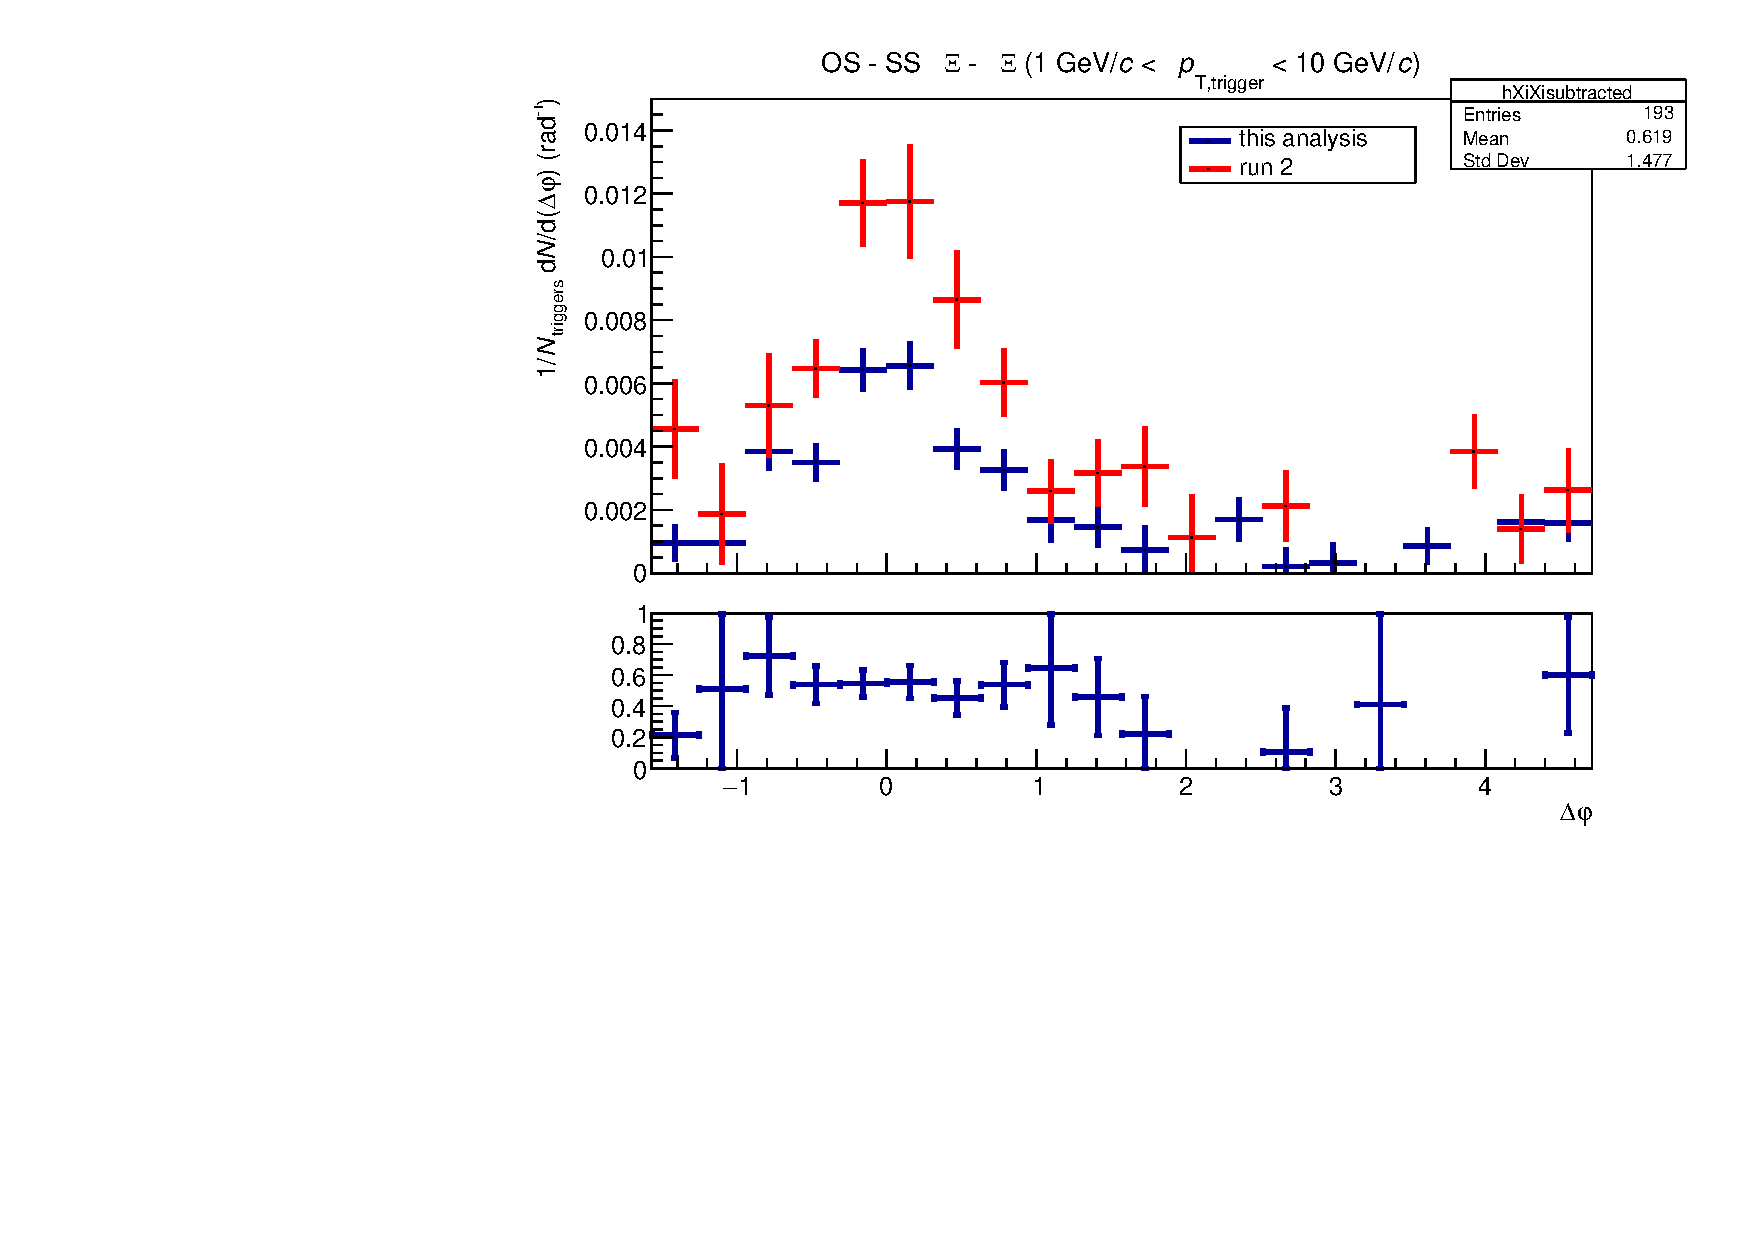
\includegraphics[width=\textwidth]{figures/Methodology/Run2Ratio.pdf}
%     \caption{Subtracted}
%     \label{fig:XiXiSub1D}
%   \end{subfigure}
%   \caption{\Xi\ - \Xi\ correlation results, combined into OS, SS, and subtracted}
%   \label{fig:results1D}
% \end{figure}

\section{Discussion}

  To place the results in context of the current understanding of hadronisation mechanisms, we compare the results to the predictions of various models. These models are all different tunes of the PYTHIA event generator, based on the Lund string fragmentation model, but each with different and/or additional mechanisms pertaining to strangeness and/or baryon production. We have reviewed these extension in some depth in Chapter \ref{ch:theory}. The Monash tune \cite{MonashTune} is the default tune of PYTHIA, which is well known to poorly describe strange baryon production.\footnote{Even the abstract of the paper introducing this tune states that ``interesting discrepancies remain in particular for strange particles and baryons'' \cite{MonashTune}.}. The Junctions \cite{Junctions} mechanism introduces new string configurations allowing for another way of producing baryons. The Ropes \cite{Ropes} model adds colour ropes, essentially allowing overlapping strings to pool their potential energy, thereby reducing the suppression of strange (di)quark production. This requires space-time modelling of the string fragmentation, which is computationally expensive and contradictory to the default momentum space in which PYTHIA normally handles the fragmentation. The Closepacking \cite{Closepacking} model attempts to generalise and extend this idea to momentum space, treating the interactions between strings as an ``effective background'' for each string. It also adds a destructive interference effect which is expected to reduce the diquark production rate. For all of the models a list of the parameters added and altered with respect to the default (Monash) settings can be found in the Appendix. 

  In May of 2025 it was reported that a bug was found in the PYTHIA code, affecting all versions of PYTHIA 8 before the discovery. \cite{PYTHIABugFix} Though this bug is not expected to have severe effects overall, it does unfortunately affect the production of baryons, and is therefor extremely relevant for our analysis. Though we have produced all the model predictions with the updated, fixed version of PYTHIA, the tunes themselves were derived with older versions that include the bug. These settings are hence not optimised for the current version of PYTHIA, and it is expected that this has an effect on the predictions of the models. This should be kept in mind when comparing the models to the data, and to each other. One exception to this is the Closepacking model, which was introduced after the bugfix, though here any setting propagated through via the default Monash tune may still be affected by the bug. 

  We report the predictions of the models for OS, SS correlation functions in Figure \ref{fig:MCXiXi} with the data analysis results for comparison. The Balance Function is presented in Figure \ref{fig:MCXiXiSubIntegral}, together with the integrated yields over the near-side, away-side, and full region. Immediately it is clear that none of the models are able to accurately describe the data, with all models overestimating the near-side peak in the OS correlation function. The Monash tune is particularly egregious, which should not come as a complete surprise, while each model that extends the fragmentation mechanisms in some way seems to do improve the correspondence. Both Monash and Junctions underestimate the pedestal as can be seen in the SS correlation function, while Ropes and Closepacking qualitatively describe the pedestal. The Closepacking model even seems to exhibit a slight dip in the near-side region of the SS correlation function compared to the away-side, though the statistical uncertainties are too large to draw any quantitive conclusions on this. Nevertheless it is a promising sign. In the Balance Function given by OS - SS all models drastically overestimate the near-side peak, while vanishing in the away-side region. This is quantified by integrating the yields over the different regions as shown in Figure \ref{fig:IntegralXiXi}. These yields may be interpreted like a probability of having a \Xi\ baryon balanced by a \Xi\ antibaryon (or vice versa) within the kinematic acceptance used in this analysis. It is clear that the vast majority of the strangeness is balanced locally, as the near-side yield is much higher than the away-side yield. 

  \begin{figure}[ht!]
    \centering
    \begin{subfigure}[t]{.49\textwidth}
      \centering
      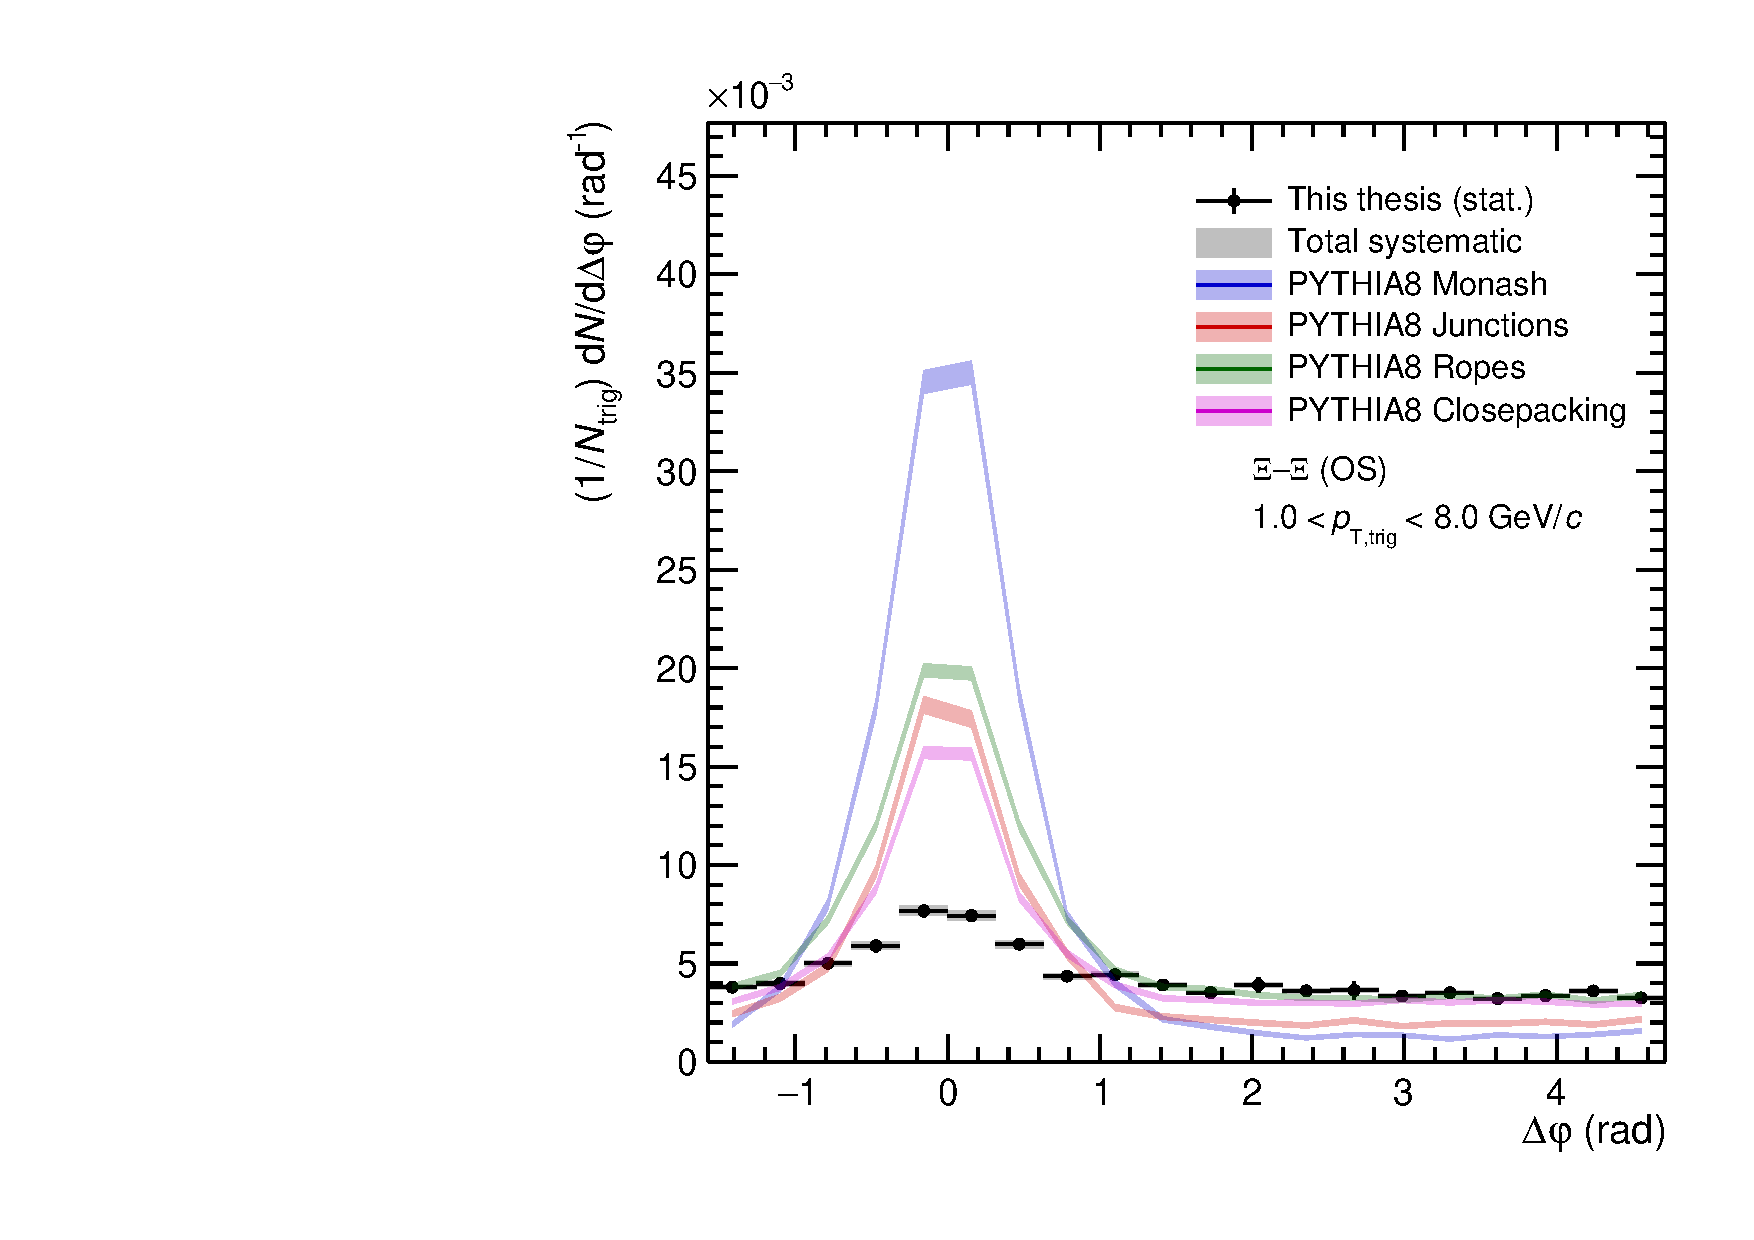
\includegraphics[width=\textwidth]{figures/Modelstudy/modelComparison_xi_xi/OS_pT_1.0_8.0.pdf}
      \caption{OS}
      \label{fig:MCXiXiOS}
    \end{subfigure}
    \hfill
    \begin{subfigure}[t]{.49\textwidth}
      \centering
      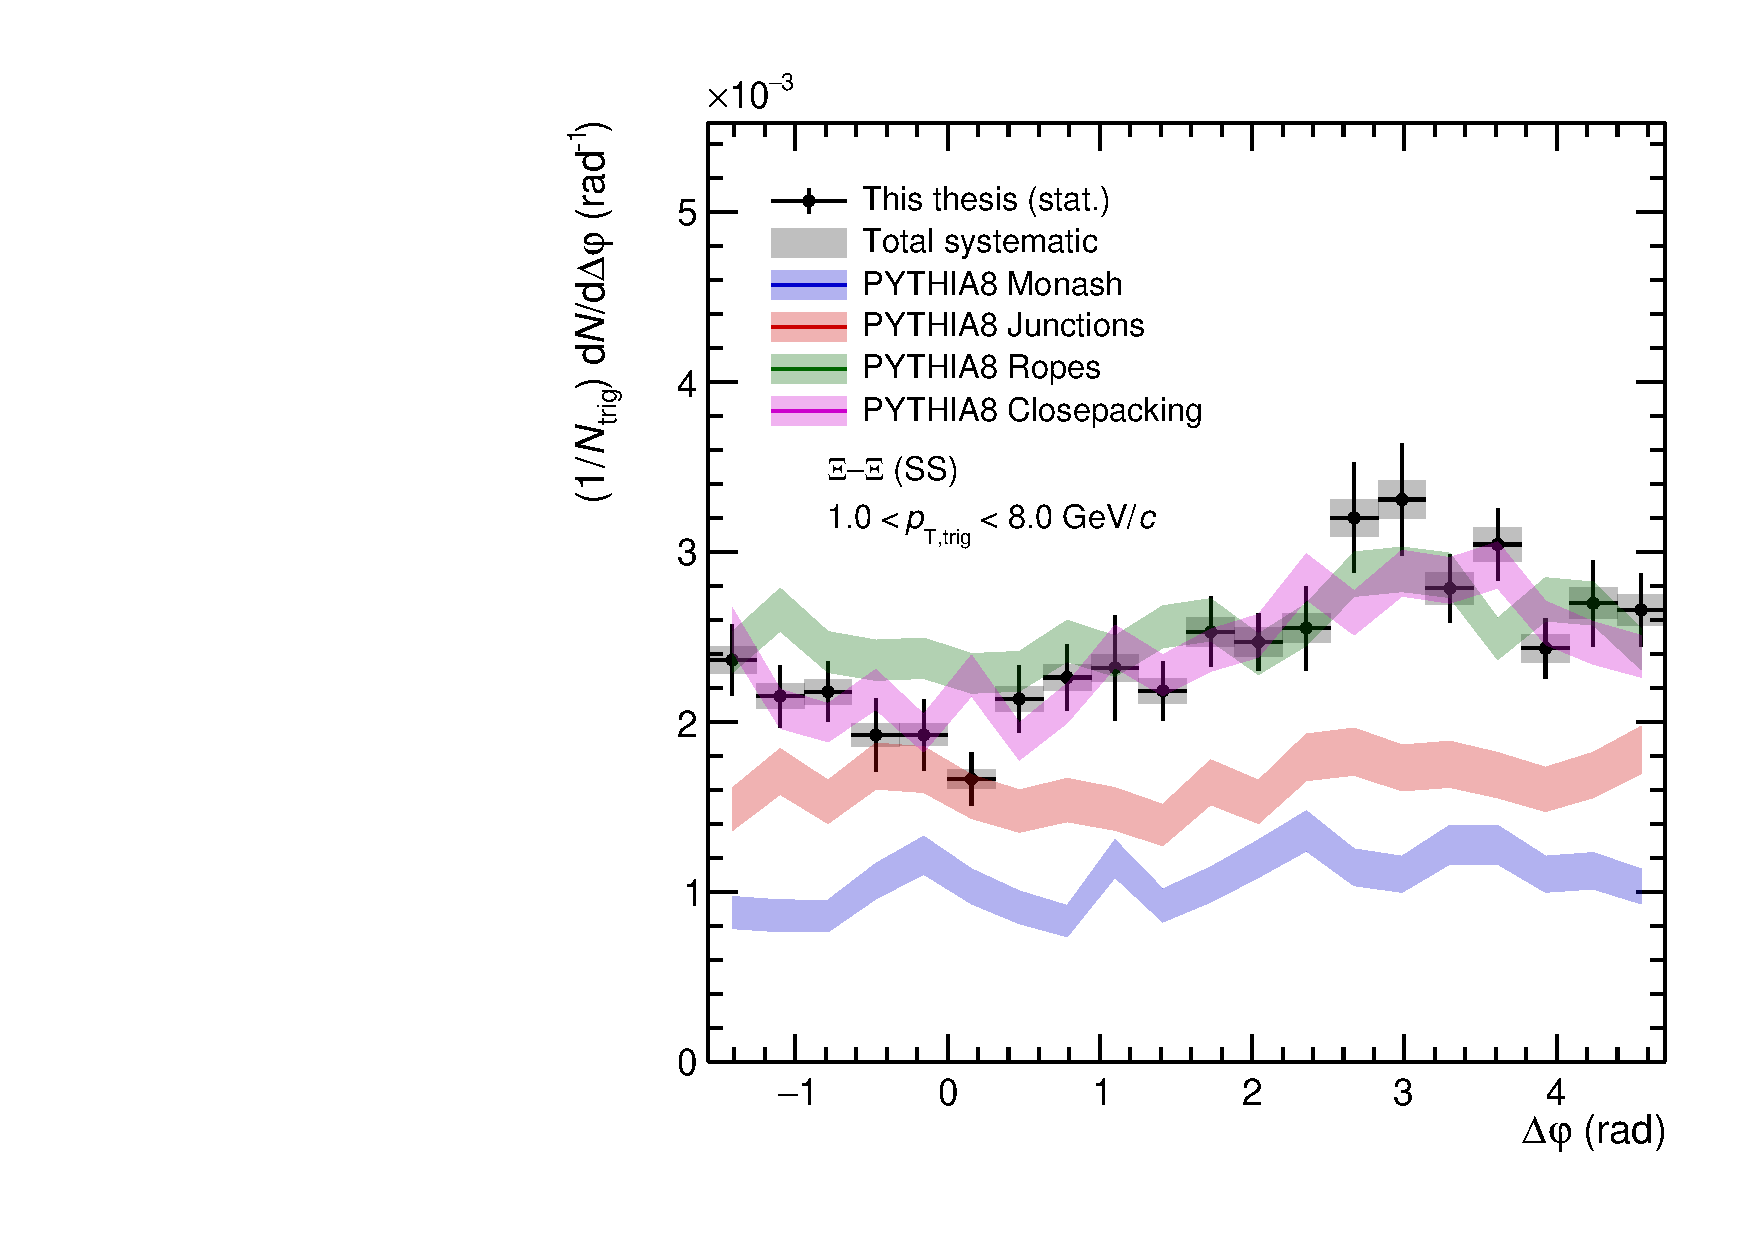
\includegraphics[width=\textwidth]{figures/Modelstudy/modelComparison_xi_xi/SS_pT_1.0_8.0.pdf}
      \caption{SS}
      \label{fig:MCXiXiSS}
    \end{subfigure}
    \caption{Model comparisons for $\Xi$--$\Xi$, $1 < \pt < 8$~GeV/$c$.}
    \label{fig:MCXiXi}
  \end{figure}

  \begin{figure}[ht!]
    \centering
    \begin{subfigure}[t]{.49\textwidth}
      \centering
      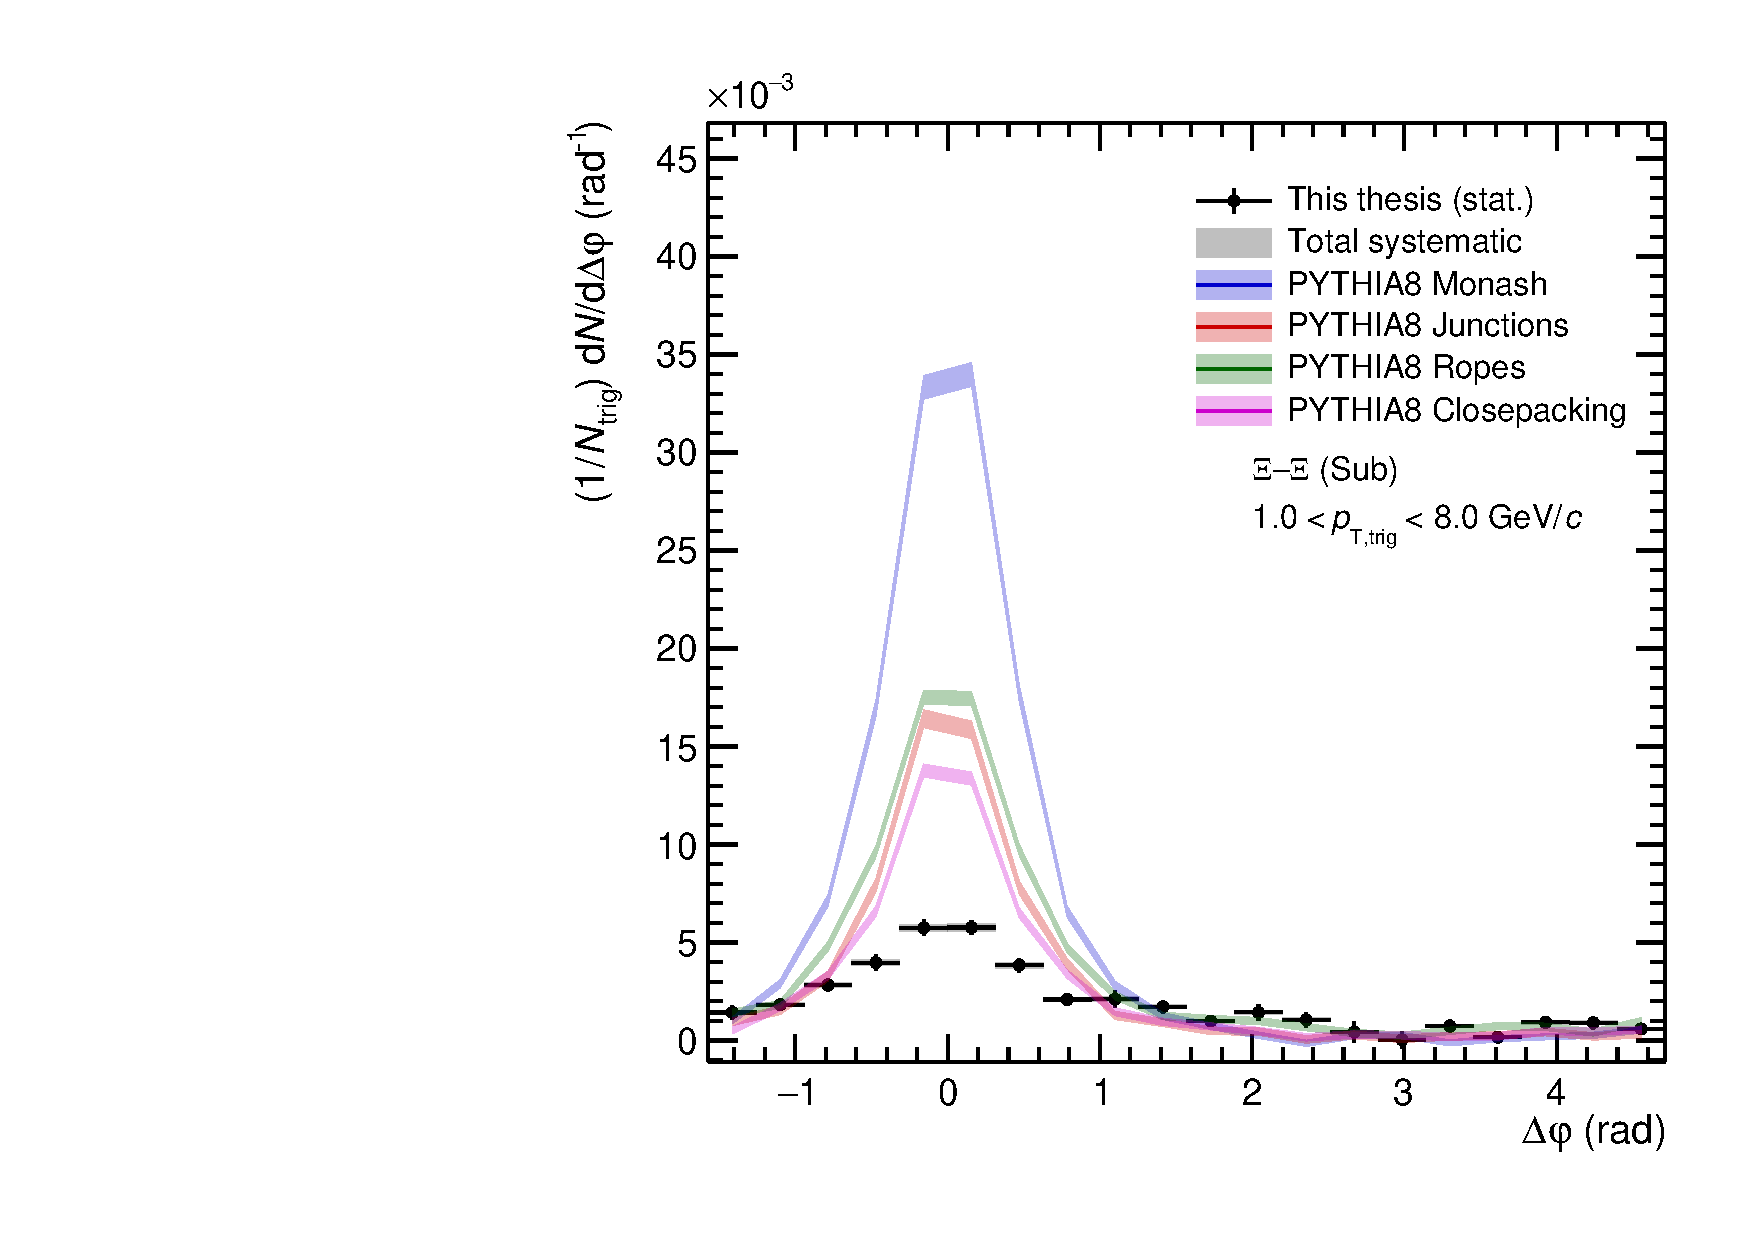
\includegraphics[width=\textwidth]{figures/Modelstudy/modelComparison_xi_xi/Sub_pT_1.0_8.0.pdf}
      \caption{\Xi\ - \Xi\ balance function.}
      \label{fig:MCXiXiSub}
    \end{subfigure}
    \hfill
    \begin{subfigure}[t]{.49\textwidth}
      \centering
      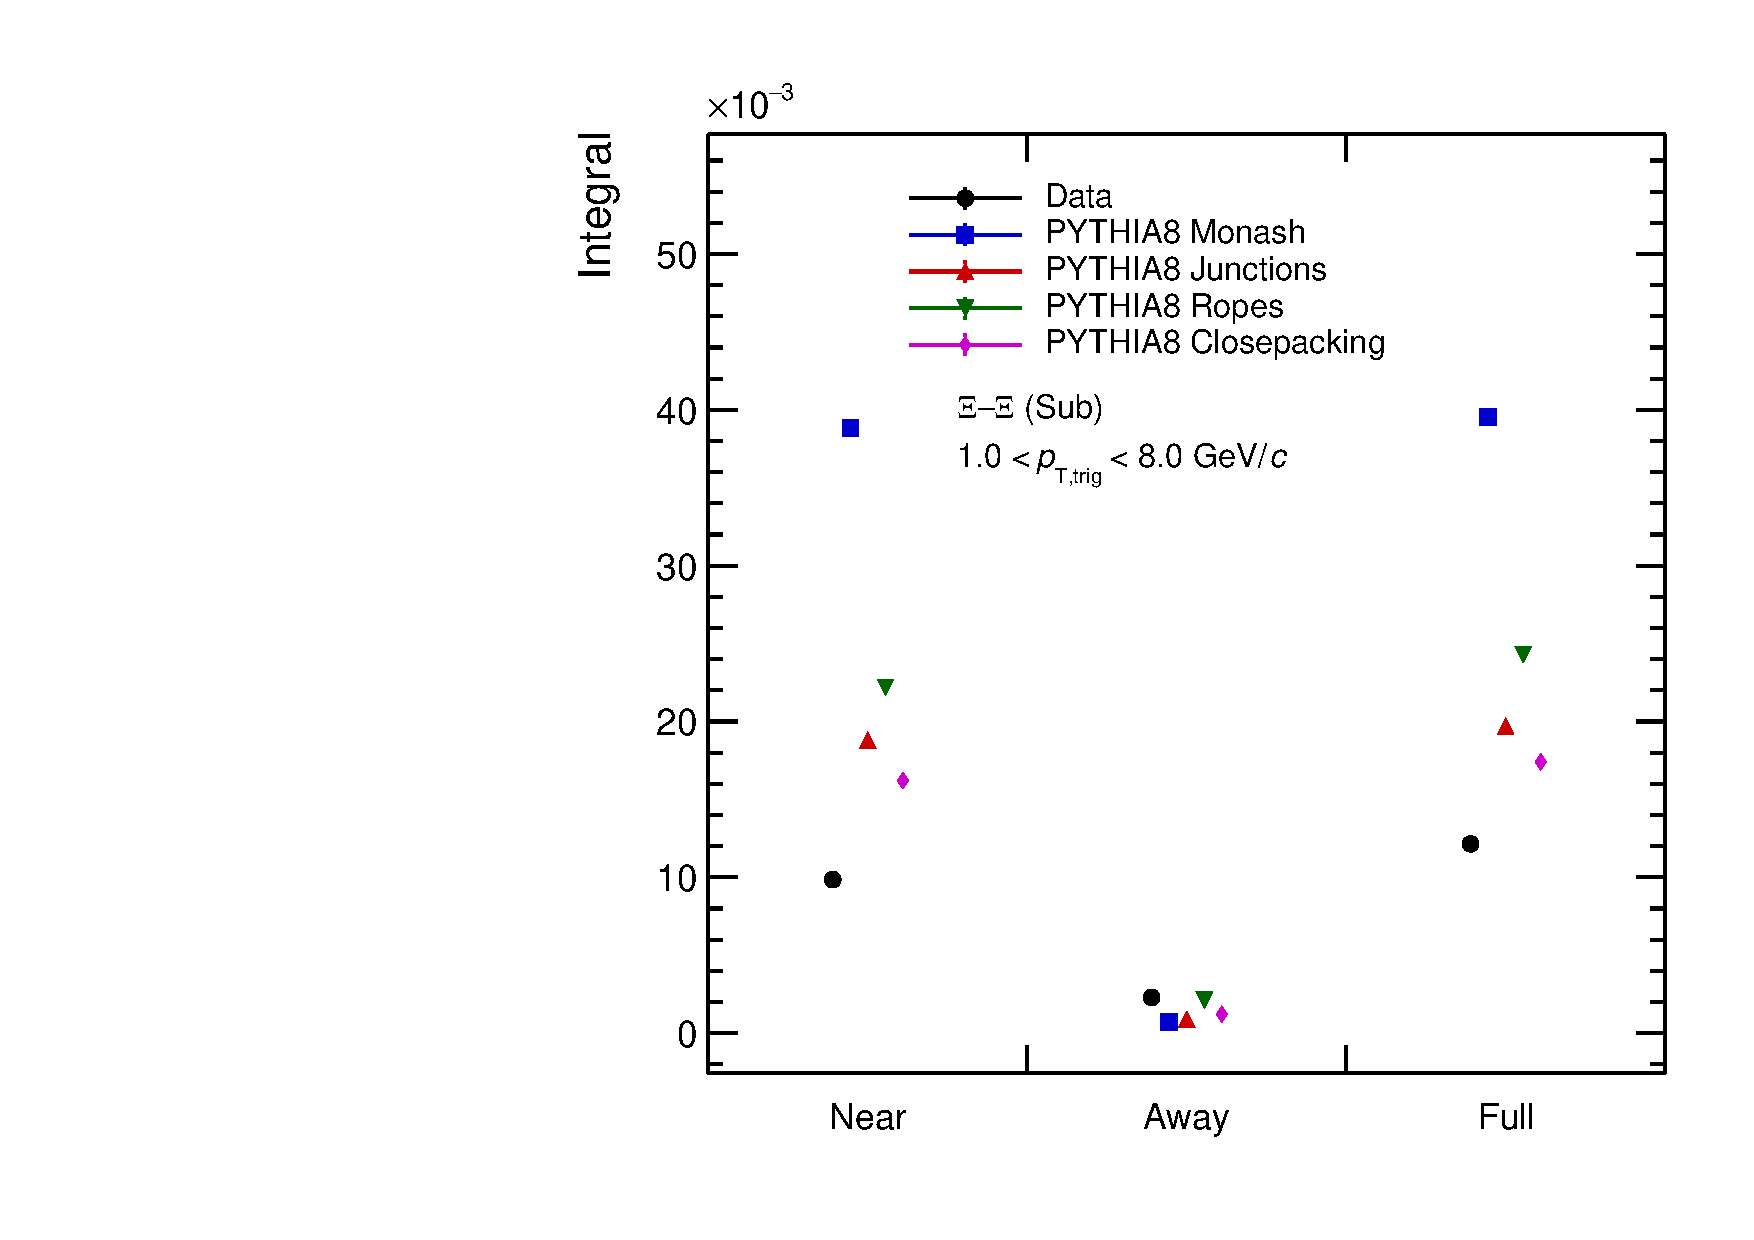
\includegraphics[width=\textwidth]{figures/Modelstudy/integralPlots_xi_xi/Sub_pT_1.0_8.0.pdf}
      \caption{Integral }
      \label{fig:IntegralXiXi}
    \end{subfigure}
    \caption{The Balance Function for \Xi\ - \Xi\ correlations in data together with various model predictions. The datapoints have both systematic and statistical uncertainties, while the model bands correspond to the statistical uncertainties only. On the right are the integrated yields for different \dphi\ regions in the reported kinematic window, where only the statistical uncertainties are shown for data and models alike. \rs{subcaptions to be removed? arguably keep the letter indices for easy referencing}}
    \label{fig:MCXiXiSubIntegral}
  \end{figure}

  We briefly return to the comparison of our analysis to the previously published results from Run 2, as shown in Figures \ref{todo} and \ref{fig:OS,SS,Sub} in Chapter \ref{ch:intermezzo}. The preceding analysis finds comparable differences between the data and several models as we do, though the discrepancy between the two data analyses persists. This of course indicates that there are significant differences in the analysis procedure, as discrepancies show up in both the data analysis as well as the model predictions. It should be noted here that, in contrary to this analysis, the model predictions in the run 2 analysis are produced with the older, bugged version of PYTHIA, which may explain some of the differences. Considering that we have verified consistent implementations of the observable definition and analysis procedure by studying the \Xi\ baryon \pt\ spectrum and performing a MC closure test for the correlation analysis, we are confident in our results. \rs{should I rephrase this? and/or should I move this to the conclusion?}

  \subsection{Omega correlations}

  Though the data analysis of this thesis is limited to \Xi\ - \Xi\ correlations, we have investigated the predictions of the models for correlations between \Xi\ and \Omega\ baryons, and between two \Omega\ baryons. Even if comparisons with data are not available yet, the behaviour of the models may differ for other species combinations, which could provide insights into the production mechanisms at play. We compare the predictions for the balance functions of all four combinations of cascade pairs in Figure \ref{fig:MCcompSub}. Note that the requirement of $p_\text{T,trigger} > p_\text{associate}$ is not applied to the \Xi\ - \Omega\ and \Omega\ - \Omega\ correlations, as the ambiguity between trigger and associate is here resolved by the species. This does have implications for the interpretation of the yields, as the release of this requirement essentially corresponds to a factor of 2, in much the same way we argued at the start of Chapter \ref{ch:intermezzo}. In any case, one should be careful comparing the yields between the different species combinations, because effects due to the kinematic boundaries may be different for the different species. For instance, if the \Omega\ baryon \pt\ spectrum is harder than the \Xi\ spectrum, then one may expect to find (relatively) more \Omega\ baryons simply as a consequence of the minimum $\pt > 1$~GeV/$c$ requirement. Accordingly, comparing the yields for any given model between \Xi\ - \Xi\ and \Xi\ - \Omega\ would not be completely fair.  
  By examining the \Xi\ - \Omega\ correlations in Figure \ref{fig:MCcompXiOmega} we immediately see a deviation from the \Xi\ - \Xi\ case, with the Ropes tune now predicting the highest near-side peak, as well as a non-vanishing away-side yield. The fact that Monash no longer predicts a much larger near-side peak than the other models can be understood as a consequence of the di-quark production mechanism. In order for a \Xi\ baryon to be balanced by an \Omega\ baryon, the string must have fragmented via the production of an $ss - \overline{s}\overline{s}$ diquark pair, which is heavily surpressed due to the high mass. On the other hand, a \Xi\ associate may be produced by either a single or double strange diquark pair. The Junctions and Closepacking models predict the lowest near-side peak and therefor yield, which could be explained by the the addition of the junction mechanism providing alternative ways of balancing the strangeness where the flavour correlation is not as strong, and fragmentation via strange (di)quarks is still suppressed. Interestingly, Closepacking predicts a correlation function comparable to Junctions, indicating that the higher effective string tension in the Closepacking model might be offset by the destructive interference effect which reduces the diquark production rate. 

  Turning our attention to the \Omega\ - \Xi\ and \Omega\ - \Omega\ correlations in Figures \ref{fig:MCcompOmegaXi} and \ref{fig:MCcompOmegaOmega}, we see that we regain similar behaviour to the \Xi\ - \Xi\ case, with Monash showing the highest near-side peak by a large margin and Closepacking the lowest. This is likely due to a similar mechanism as outlined for the \Xi\ - \Omega\ case: in Monash, an \Omega\ baryon trigger implies that the string has framgented via the production of an $ss - \overline{s}\overline{s}$ diquark pair, which immediately means that the balancing hadron must contain at least two strange quarks as is the case for \Xi\ and \Omega\ baryons. Though the there are some slight differences for the other models, the qualitative behaviour seems to be similar to the \Xi\ - \Xi\ case, considering the ordering of the models from highest to lowest near-side peak is the same. It would still be very interesting to investigate ratios between different models as there are some differences there, while the ratios are more robust against effects related to the kinematic boundaries. For instance, the ratio between heigths of the peaks of the Closepacking and Monash models is different for the \Xi\ - \Xi\ and \Omega\ - \Xi\ cases, which could probe the additional hadronisation mechanisms while taking the pure diquark production in Monash as a baseline. 

  \rs{perhaps do include the yield plots as well, so we may compare the relative yields per species combination. e.g. closepacking/monash seems much lower for omega-xi than xi-xi, while we do regain much of the xi-xi behaviour in that case. maybe do integral plots in logscale anyway?}

  \begin{figure}[ht!]
    \centering
    \begin{subfigure}[t]{.49\textwidth}
      \centering
      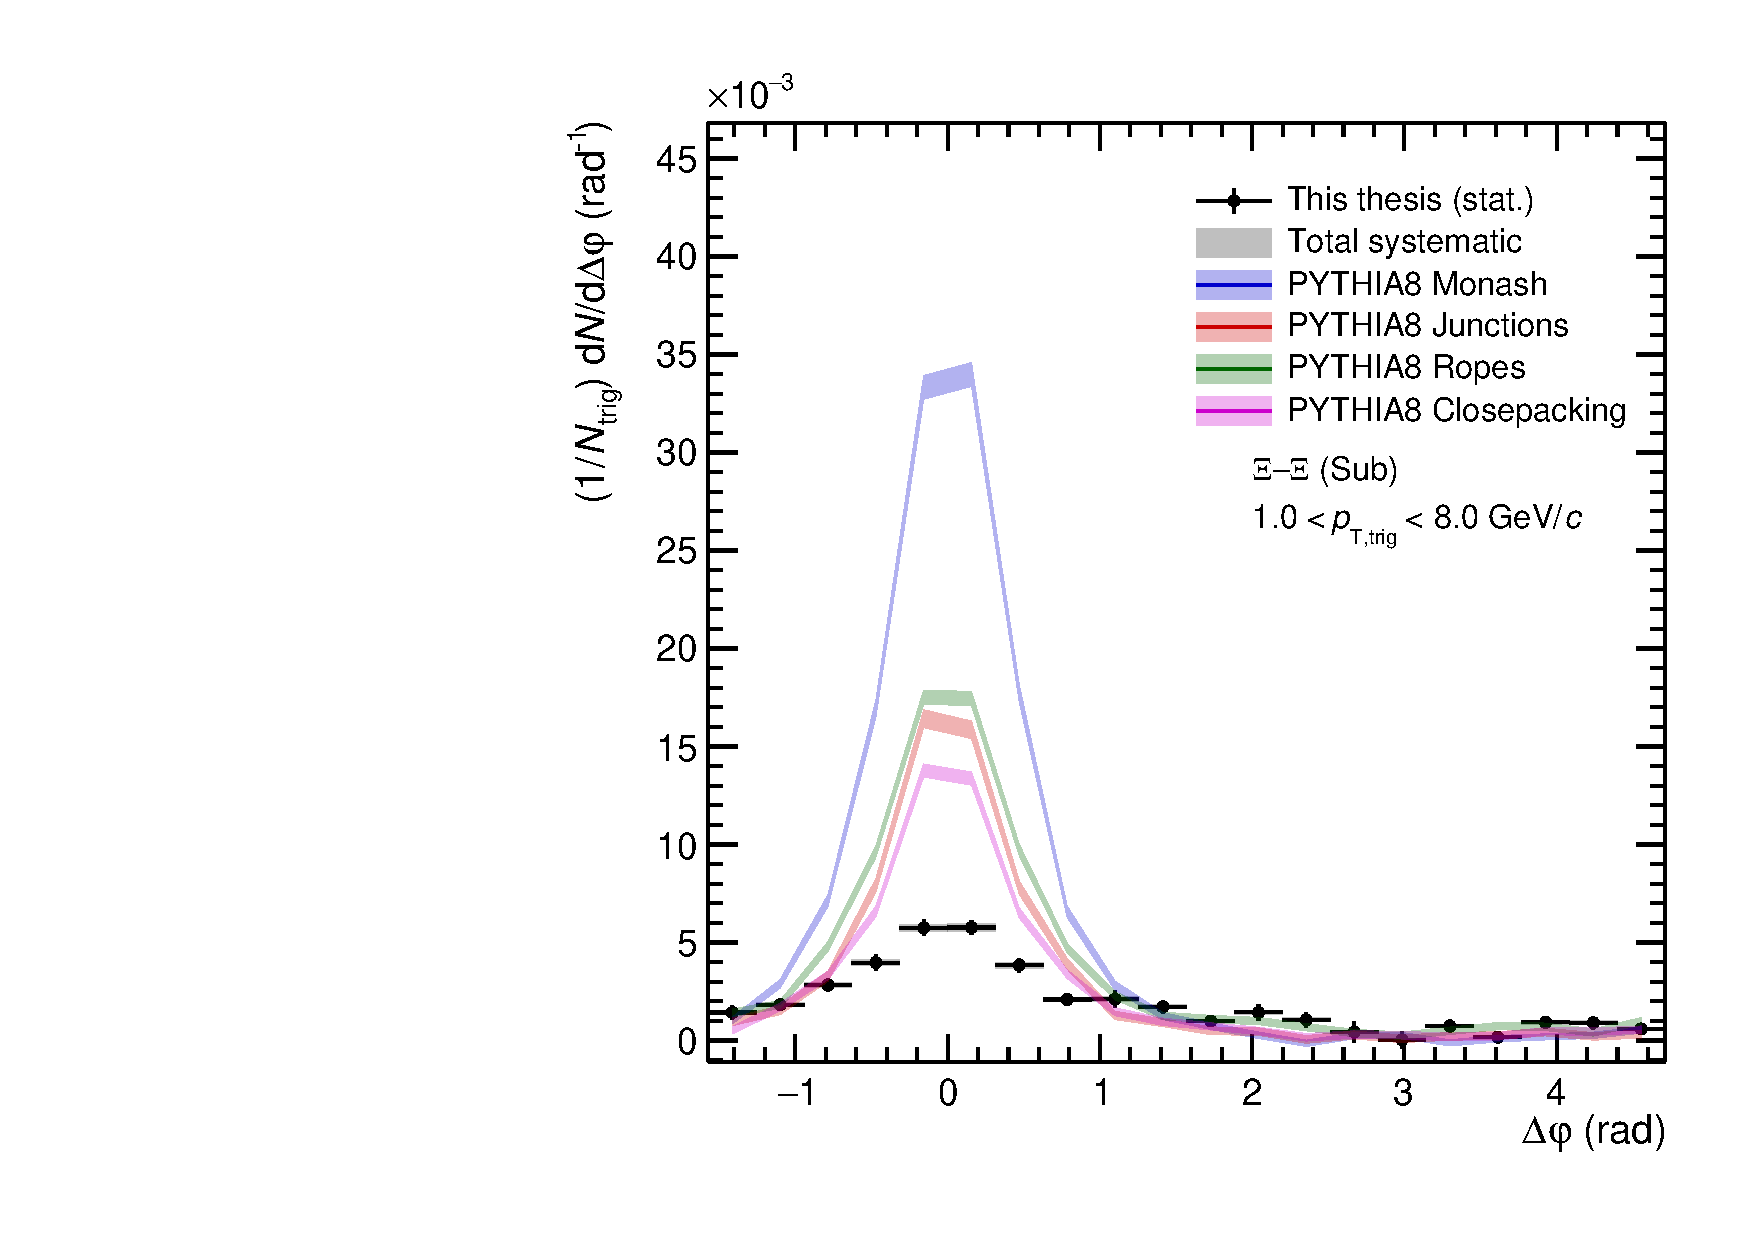
\includegraphics[width=\textwidth]{figures/Modelstudy/modelComparison_xi_xi/Sub_pT_1.0_8.0.pdf}
      \caption{\Xi\ - \Xi\ balance function.}
      \label{fig:MCcompXiXi}
    \end{subfigure}
    \hfill
    \begin{subfigure}[t]{.49\textwidth}
      \centering
      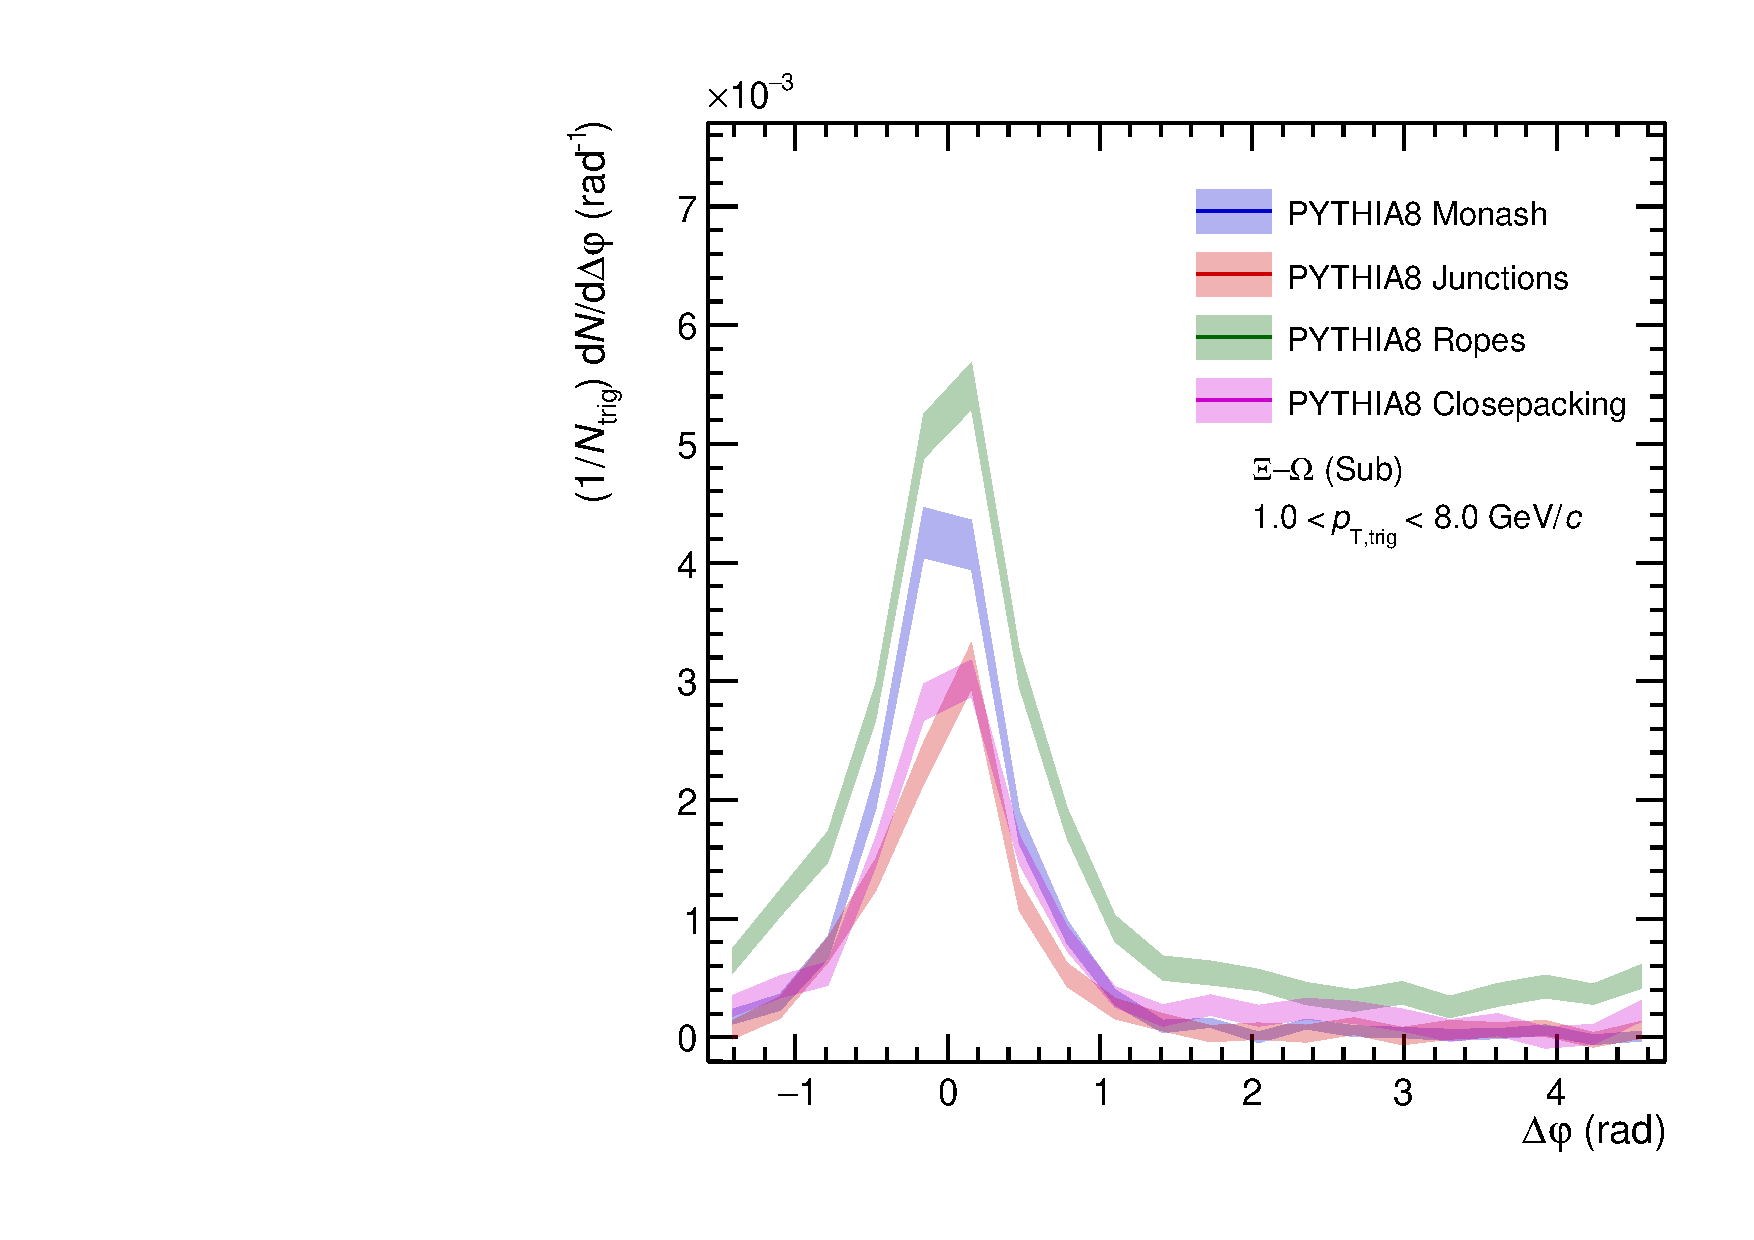
\includegraphics[width=\textwidth]{figures/Modelstudy/modelComparison_xi_omega/Sub_pT_1.0_8.0.pdf}
      \caption{$\Xi$--$\Omega$}
      \label{fig:MCcompXiOmega}
    \end{subfigure}
    \begin{subfigure}[t]{.49\textwidth}
      \centering
      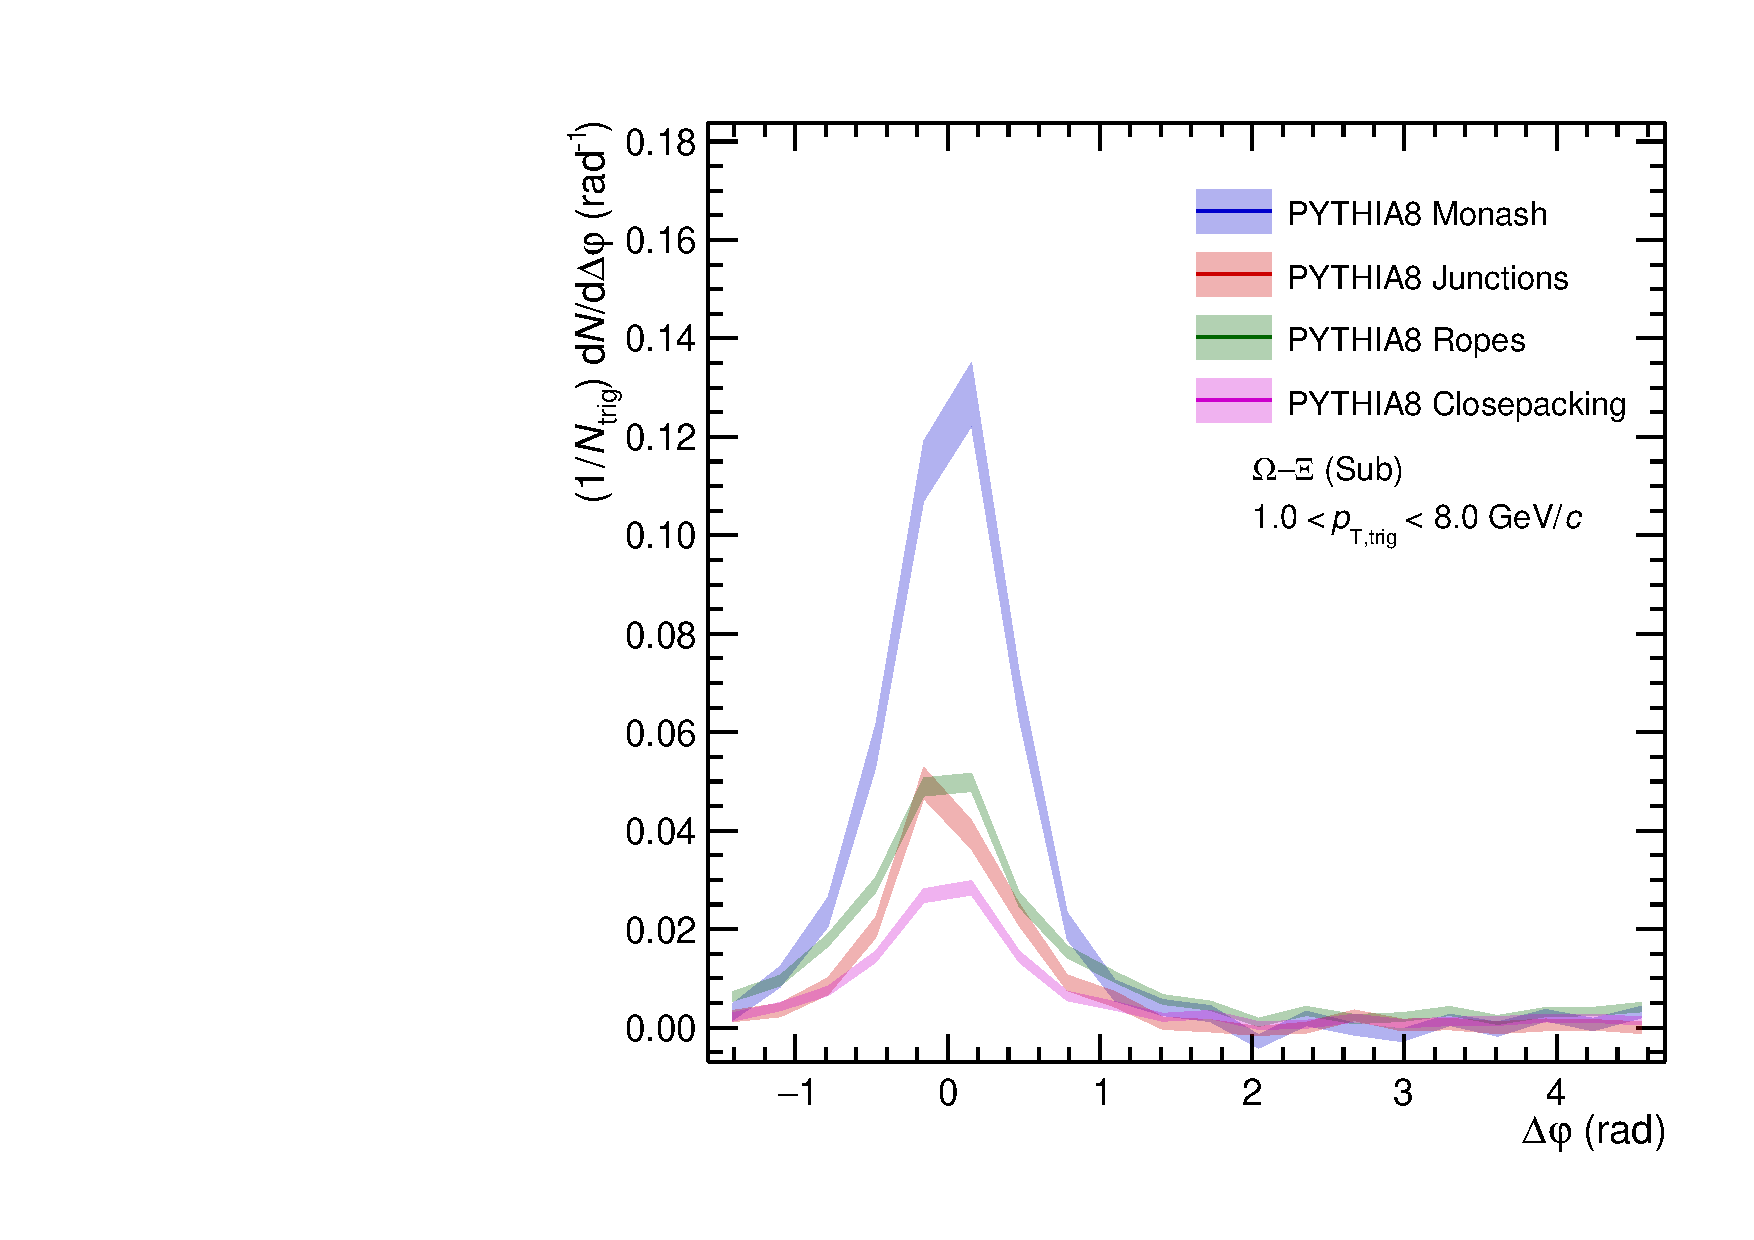
\includegraphics[width=\textwidth]{figures/Modelstudy/modelComparison_omega_xi/Sub_pT_1.0_8.0.pdf}
      \caption{$\Omega$--$\Xi$}
      \label{fig:MCcompOmegaXi}
    \end{subfigure}
    \hfill
    \begin{subfigure}[t]{.49\textwidth}
      \centering
      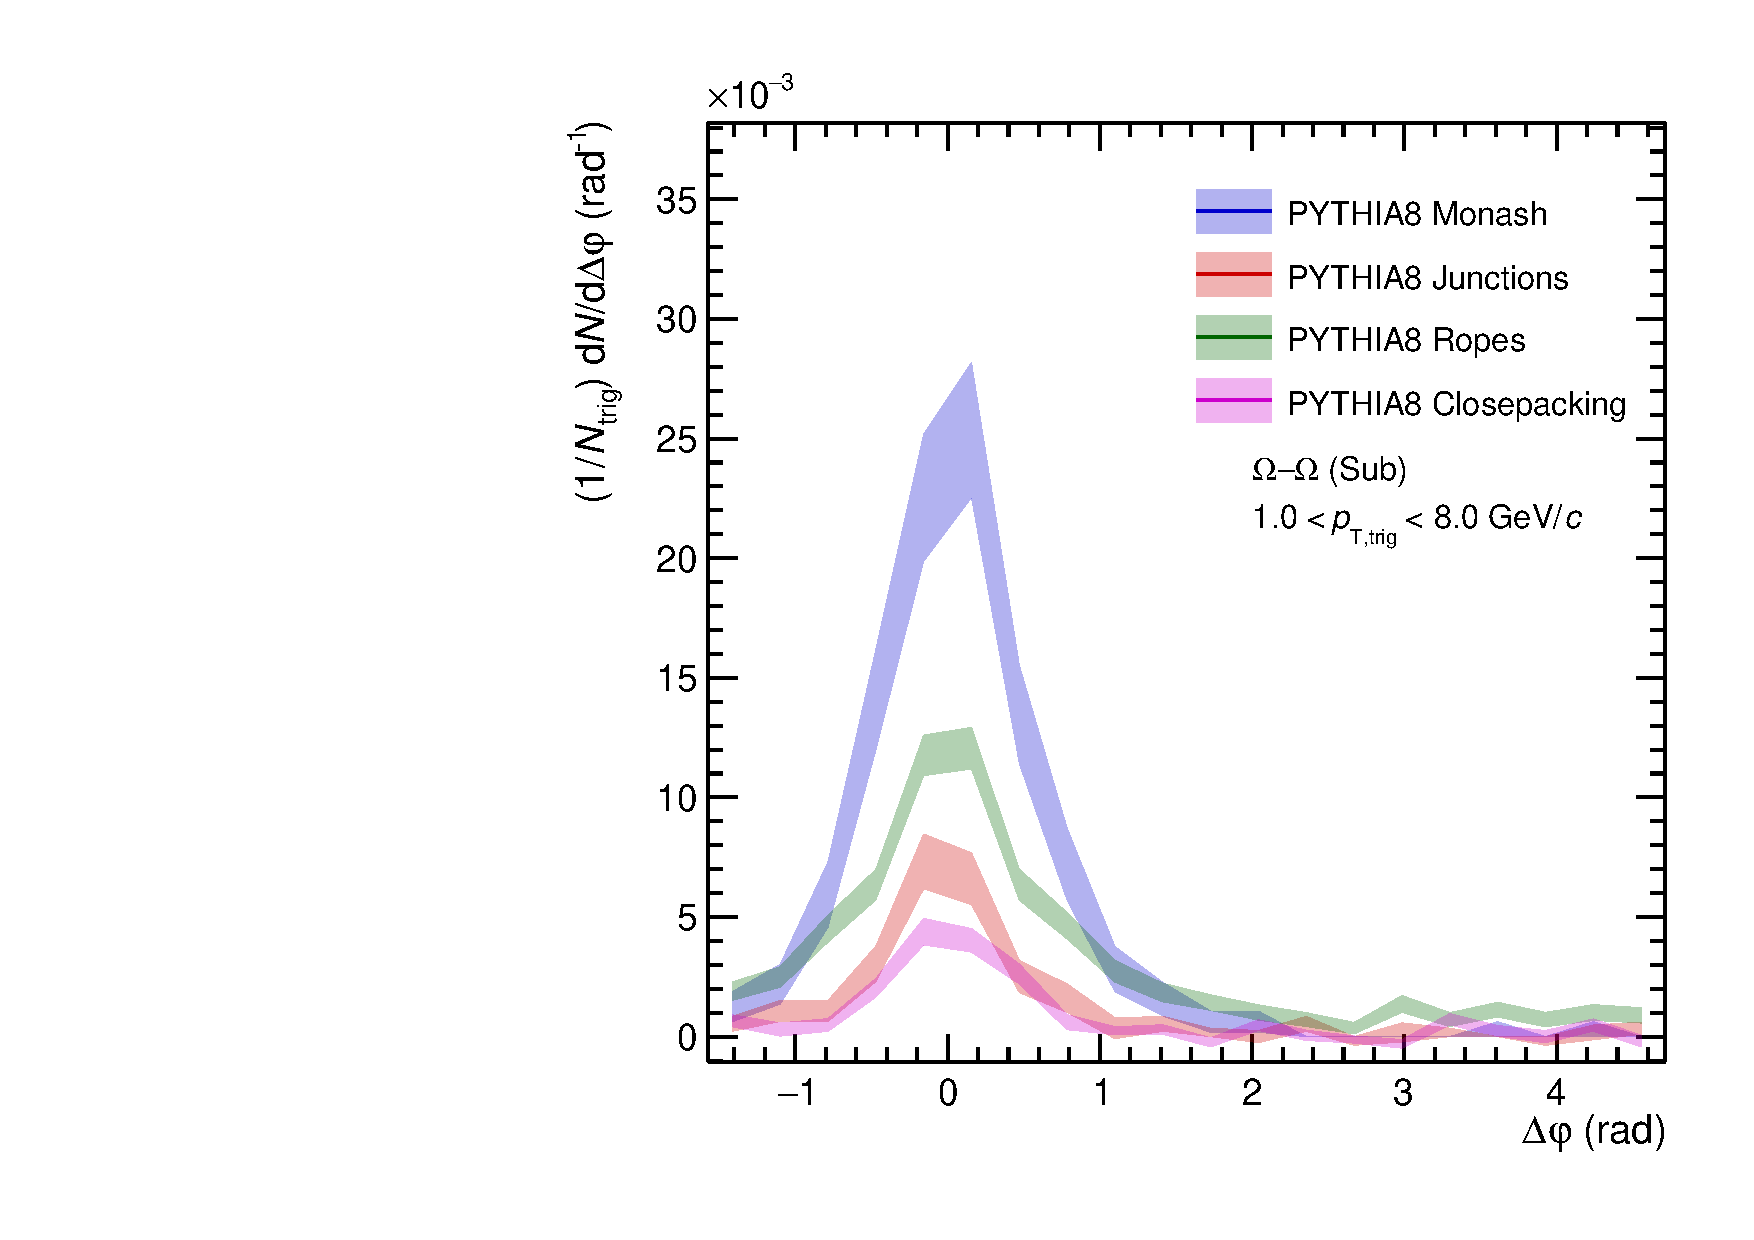
\includegraphics[width=\textwidth]{figures/Modelstudy/modelComparison_omega_omega/Sub_pT_1.0_8.0.pdf}
      \caption{$\Omega$--$\Omega$}
      \label{fig:MCcompOmegaOmega}
    \end{subfigure}
    \caption{Balance function model comparisons for all combinations. \rs{improve histo caption, remove subcaptions.}}
    \label{fig:MCcompSub}
  \end{figure}

\section{Conclusion/outlook}

  We have presented the correlation functions for \Xi\ - \Xi\ pairs in pp collisions at $\sqrt{s} = 13.6$ TeV for \Xi\ baryons with $1 < \pt < 8$~GeV/$c$, together with predictions from various models. The results show a clear near side peak on top of a pedestal in the OS correlation function, while the SS correlation function only exhibits the pedestal and a small near-side dip. All models vastly overestimate the near side peak to varying degrees, with models that extend the fragmentation mechanisms generally performing better than the default Monash tune. The Ropes and Closepacking models qualitatively describe the pedestal, while Monash and Junctions underestimate it. The Closepacking model even seems to exhibit a slight dip in the near-side region of the SS correlation function compared to the away-side, though the statistical uncertainties are too large to draw any quantitive conclusions on this. In the Balance Function given by OS - SS all models drastically overestimate the near-side peak as given by the OS correlation function, while vanishing in the away-side region. This is quantified by integrating the yields over the different regions, which shows that the vast majority of the strangeness is balanced locally, as the near-side yield accounts for almost all of the yield within the kinematic acceptance used in this analysis. 

  Expanding the scope of the current analysis to also include correlations between \Xi\ and \Omega\ baryons, as well as between two \Omega\ baryons, would provide further insights into the hadronisation mechanisms at play. Especially comparing results between correlations that have the same trigger but different associate species may prove valuable, which is further motivated by the observation that model predictions are quite different for the \Xi\ - \Omega\ case compared to the \Xi\ - \Xi\ case. \Omega\ - \Omega\ correlations may prove particularly statistically challenging, though the existence of ``triggered'' (also known as ``skimmed'') datasets could be very helpful in this regard, as they allow for storage of only relevant events. Another avenue worth exploring is the multiplicity dependence of the correlations. It is well known that strangeness production is enhanced in high multiplicity pp collisions, and it would be interesting to see how the correlations evolve with multiplicity, especially in the context of the different models. 

  While extensions of the Lund string model seem to improve the description of the data in various strangeness analyses, none of the models are able to quantitatively describe the data in this analysis. This indicates that the hadronisation process of strange baryons is not captured in the existing models, least of all understood. Retuning the models with the fixed version of PYTHIA is needed to further understand the discrepancies between the models and the data, as well as between the models themselves. Still, there is no guarantee that any retuning will improve the description of the data. 

  It is a really challenging task to understand soft QCD processes, where hadronisation is an important facet. From the theoretical and phenomenological point of view, calculations from first principles are nigh impossible, and even simplified models can quickly become convoluted. On the experimental side, soft QCD processes can only be probed indirectly via measurements of the final state hadrons that cannot be unfolded back to the partonic level. Iterations between theory, models, and experiments have proved to be a fruitful way to advance our understanding of particle physics, and this is what we attempt as well. In the context of soft QCD processes this is complicated by the fact that the models require significant input from experiments to be tuned, making it harder to draw conclusions from comparisons between models and data. After all, when designing a model to specifically reproduce (some aspects of) data, one should be careful to not over-interpret the agreement between the model and the data, as it may be a consequence of the tuning rather than a consequence of the physics mechanisms included in the model. On top of this, while adding mechanisms may have valid physical motivation, adding free parameters to a model generally makes it easier to fit the data, but harder to interpret the physics behind the model. In any case, the discrepancies between the data and the models in this analysis indicate that there are still important aspects of the hadronisation process that we do not understand. Further research on both the phenomenological and experimental side is needed to advance our understanding of hadronisation, and since the strange baryon sector is arguably the least understood sector of hadronisation, it is a very promising avenue to explore.

  \rs{I will think about how to extend this myself, as my writing inspiration has run out at the moment. Any thoughts on what to discuss in the results/discussion/conclusion/outlook sections are very welcome!}


\appendix

\chapter{MC closure}
\label{ch:mc_closure}
\input{chapters/appendices/McClosure.tex}

\chapter{Model plot dump}
% \input{chapters/appendices/MCplotdump.tex}

\chapter{PYTHIA settings}
\label{ch:pythia_settings}
\rs{put here the pythia configurations.}

%\section{Methodology write-up}
% \input{WriteUp.tex}

% dummy citation
% This is a dummy citation to stop the compilation errors. \cite{WWW}

\printbibliography

\end{document}
